%%% use twocolumn and 10pt options with the asme2ej format
\documentclass[twocolumn,10pt]{asme2ej}

\usepackage{epsfig} %% for loading postscript figures
\usepackage[font=small,labelfont=bf]{caption}
\usepackage{enumitem}
\usepackage{amsmath} % for "bmatrix" environment and "\dfrac" macro
\usepackage{relsize}
\usepackage{float}
\usepackage{courier}
\usepackage{xcolor}
\usepackage{fancyhdr}

\usepackage{multicol}



\setlength{\parindent}{0pt}
\newcommand{\id}{\hspace{6 mm}}


%\raggedbottom

\title{Low-Cost Visible Light Spectral Imaging}

\author{Daniel W. Dichter
    \affiliation{
Independent Researcher\\
Cambridge, Massachusetts, U.S.A.\\
daniel.w.dichter@gmail.com\\
\\
\color{red}
\emph{\textbf{DRAFT: \today}}\\
\color{black}

    }	
}

\begin{document}

\maketitle

\pagestyle{fancy}

\begin{abstract}{\it Spectral imaging is an emerging technology for measuring spectral power distributions (SPDs) of electromagnetic radiation over a two-dimensional spatial domain. Within the visible light wavelength band, spectral imaging measures light and color with greater accuracy than digital photography. However, high cost limits its accessibility. Accordingly, a low-cost method is developed using commercially-available hardware --- primarily a DSLR camera and a set of narrow bandpass filters. The quantity of filters is minimized to a total of seven, set by the dimensionality of SPDs, the spectral sensitivities of eyes and cameras, and commercial availability. Camera spectral sensitivity is measured using this same filter set, a color chart, a spectrophotometer, and noon daylight modeled as CIE D65. The RAW photo format is used to access unprocessed sensor data. Independent SPD measurements from each color channel are fused as a sensitivity-weighted average for efficient and continuous interpolation between color channels with a high signal-to-noise ratio. Images are reconstructed from SPDs with standard observer functions. The method is demonstrated with a Canon 650D camera, a set of Thorlabs one-inch narrow bandpass filters, an X-Rite ColorChecker chart, and a Spectro 1 spectrophotometer. Accuracy is validated by quantitative comparison against ground truth measurement. The total filter cost is \$715, plus \$405 to measure camera sensitivity.}
\end{abstract}

\section{Introduction}

\subsection{Background}

% Motivate spectral imaging generally

Color perception results from the interaction of an illuminant, optionally a reflective surface, and an observer. Humans are trichromats, having three-dimensional color perception, over the visible light wavelength spectrum of 400 to 700 nm. Human color perception is significantly rank-deficient even within its wavelength limits, as shown in Sections \ref{dimensionality} and \ref{curve_reconstruction}.

% Overview of hyperspectral datacubes

\id Whereas digital photography produces a three-dimensional RGB (red, green, blue) color image, spectral imaging produces an $k$-dimensional hyperspectral datacube (HSDC), typically with 10 $\leq$ $k$ $\leq$ 60; wavelength channels replace color channels. HSDCs are informationally complete and observer independent, providing a more accurate representation of color, and enabling greater optionality in subsequent image processing.

% Spectral scanning

\id Spectral scanning is the simplest of several methods of generating HSDCs, wherein a 1-channel intensity image is captured at a series of regularly-spaced, narrow, non-overlapping wavelength bands. These images are subsequently ``stacked'' to form the final HSDC. Though spatially high-resolution relative to other methods, spectral scanning experiences ``spectral smearing'' if the subjects or sensor move during the image capture process, due to the characteristically large temporal distribution of the images. By comparison, so-called ``single-shot'' methods use various diffraction techniques to capture the entire HSDC simultaneously, but at lower spatial resolution.

% Cameras

\id A survey of commercially-available hyperspectral cameras\footnote{PixelTeq SpectroCam-VIS, BaySpec GoldenEye, Resonon Pika L} showed a price range of \$20,000-25,000. Consumer cameras such as DSLRs cost 1-10\% of this amount. Consumer cameras are not capable of spectral imaging as-is, but various investigators have demonstrated this capability nonetheless with various hardware and software methods. All such methods account for the non-linear trichromate spectral sensitivity of the camera's Bayer filter and image sensor.

\subsection{Related Work}

Several authors have demonstrated spectral imaging with commercially-available cameras.

\id Cosentino \cite{Cosentino} used 12 bandpass filters to produce HSDCs, comparing results favorably to a commercial hyperspectral camera. The method requires modification of the camera, the filters are of non-uniform properties, and the quantity of filters is larger than necessary.

\id Baek et al. \cite{Baek} developed a single-shot method using a custom prism objective for diffraction grating. Combined spatial and wavelength information is separated by detection of ``spectral cues'' present ``only around object edges''. The requirement for the presence of edges limits the scenes that may be captured, and leads to a sensitive dependence between scene and system accuracy.

\id Habel et al. \cite{Habel} similarly developed a single-shot diffraction grating method. The custom objective is large and complex, and the reconstructed images are limited to 120 x 120 pixels.

\id Oh et al. \cite{Oh} developed a method using three different synchronized digital cameras, exploiting small differences in their sensitivities. An image registration process is used to align images between cameras using planarity. Principal component analysis is performed on a spectral database of Munsell colors to create a low-dimension vector space for describing SPDs as linear combinations.

\id Berns et al. \cite{Berns} used a large-format camera and an optimized set of filters. Singular value decomposition was performed on a dataset of 2,500 reflectance spectra to reduce the quantity of filters required to a total of six, showing favorable accuracy of SPDs against ground truth.

\id The method described in this paper is believed to be novel in its low cost, high spatial resolution, use of unmodified commodity hardware, and independence from training data.

\section{Methods}

\subsection{Dimensionality of Reflectance Spectra}
\label{dimensionality}

Parkkinen et al. \cite{Parkkinen} measured the reflectance spectra of 1,257 standard Munsell color chips over 400 to 700 nm. Noting that ``the components of a color spectrum are highly correlated'', the authors performed principal component analysis on these spectra, producing a set of reflectance eigenvectors. It was found that these spectra could be reconstructed as linear combinations of eight or fewer eigenvectors. This result implies that reflectance spectra are up to eight-dimensional over the visible light spectrum, with a characteristic wavelength resolution of approximately (700 nm - 400 nm) / 8 = 37.5 nm.

\subsection{Curve Reconstruction}
\label{curve_reconstruction}

Sampling an SPD by spectral scanning with narrow bandpass filters produces a sparse sample; the value of the SPD is measured only at certain regular intervals. Between these, the value of the SPD is not measured, but can be approximated due to the limited dimensionality of SPDs. This process is modeled as a curve reconstruction problem, i.e.\ given a sparse sampling of an unknown curve, reconstruct the curve by means of an appropriate interpolation scheme such that the reconstructed curve matches a theoretical measured curve. This concept is shown in Figure \ref{curve_reconstruction_colorchecker_2}.

\id To determine the optimal filter quantity and interpolation scheme, two reflectance datasets are considered: the 8 eigenvectors developed by Parkkinen et al.\ \cite{Parkkinen} with 5 nm resolution, and the 24 reflectance spectra measured from an X-Rite ColorChecker Classic \cite{X-Rite} using a Spectro 1 spectrophotometer with 10 nm resolution. The reconstruction domain is taken as [420 660] nm per Section \ref{section_filters}. The quality of the reconstruction is calculated as the residual sum of squares (RSS) for all curves, multiplied by the wavelength resolution, divided by the quantity of samples in the dataset. This calculation is performed for both reflectance spectra and simulated SPDs using D65 scaled to the range of [0 1]. This normalized error metric allows direct comparison between datasets. The filters are assumed to be of sufficiently narrow bandwidth that they measure at their exact center wavelength (CWL). The following observations were made:

\begin{enumerate}
  \item 30 nm resolution outperforms 40 nm resolution in all cases.
  \item With a 40 nm resolution, cubic interpolation is optimal.
  \item With a 30 nm resolution, cubic interpolation is at least near-optimal.
  \item Optimized error at 40 nm is 1-3x the optimized error at 30 nm, but both are small in an absolute sense.
  \item Reflectance (not illuminant) dominates the quality of the curve reconstruction.
\end{enumerate}

Thus, 40 nm resolution and cubic interpolation are used for curve reconstruction.

\begin{figure}
\centering
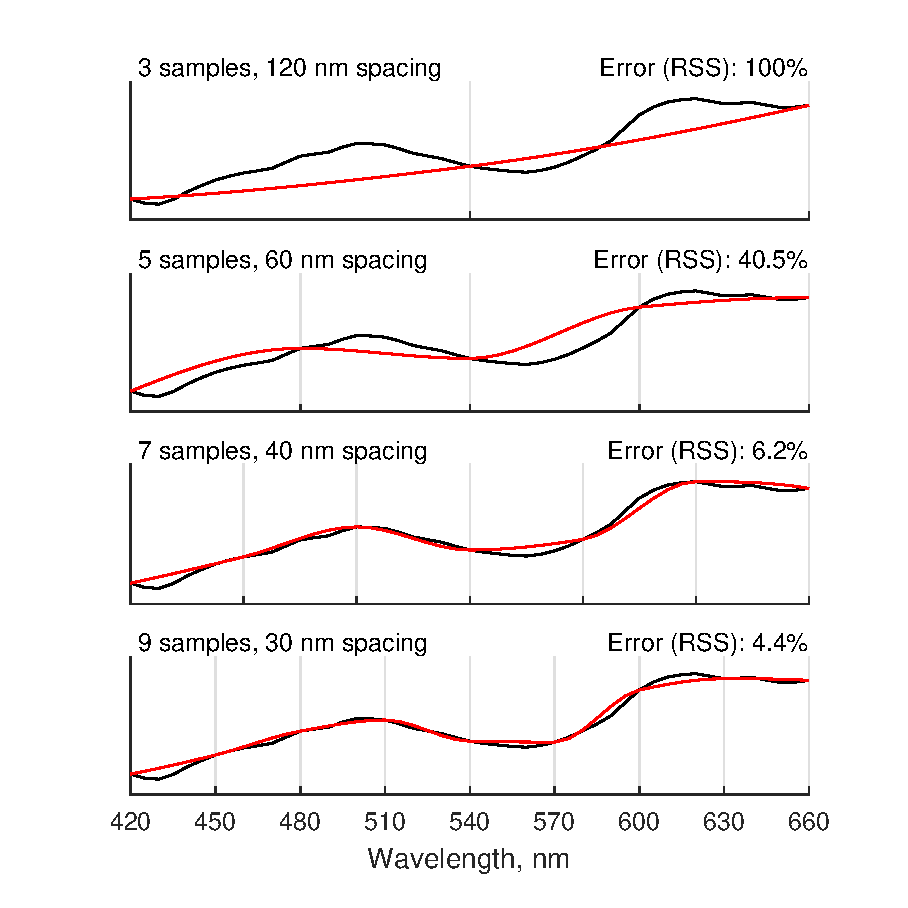
\includegraphics[width=0.5\textwidth]{curve_reconstruction_colorchecker_2.eps}
\caption{Curve reconstruction for SPD of ColorChecker swatch \#2 under D65 illuminant for varying sample quantity. Samples are denoted with vertical lines, with cubic interpolation between samples.}
\label{curve_reconstruction_colorchecker_2}
\end{figure}

\subsection{Filter Set Design}

\label{section_filters}

Manufacturers of narrow bandpass filters include Thorlabs, Edmund Optics, and MidOpt. Within the visible light spectrum, CWL is generally discretized as whole-number multiples of 10 nm, i.e.\ [400, 410, 420, ..., 700] nm.

\id The centroid of the visible light spectrum may be defined at the wavelength corresponding to 50\% on the cumulative density function (CDF) of the sum of the CIE 2° tristimulus observer functions [$\bar{x}, \bar{y}, \bar{z}$]. \cite{CVRL} Rounding to the nearest 10 nm per commercial availability, this centroid is 540 nm.

\id It can be shown that the wavelength range of 420 to 660 nm encompasses 97\% of the area under the CIE 2° and 10° observer functions, \cite{CVRL} thus:\\

$ \displaystyle \int_{\textrm{420 nm}}^{\textrm{660 nm}} ( \bar{x}+\bar{y}+\bar{z} ) d\lambda \approx \int_{-\infty}^{\infty} ( \bar{x}+\bar{y}+\bar{z} ) d\lambda $ \\

This range is also evenly divisible into 40 nm increments, and intersects the centroid of 540 nm.

\id The final specification is the full-width half max (FWHM), or bandwidth. As discussed in Section \ref{curve_reconstruction}, it is desirable to minimize FWHM so that SPD measurements are wavelength-accurate to the CWL. The reduction in overall transmission associated with a low FWHM can be compensated by increasing the exposure, as discussed in Section \ref{photographic}.

\id The set of filters chosen are shown in Figures \ref{thorlabs_filter_transmission_spectra} and \ref{canon}, and have the following properties:\\

\begin{tabular}{l | l}
%\hline
Quantity & 7 \\
Manufacturer & Thorlabs \\
CWL & 420 to 660 nm \\
CWL Spacing & 40 nm \\
FWHM & 10 nm \\
Part Numbers & FB420-10, FB460-10, etc. \\
Diameter & 1'' \\
Cost, Total & \$686 (+\$29 case) \\
%\hline
\end{tabular}

\begin{figure}
\centering
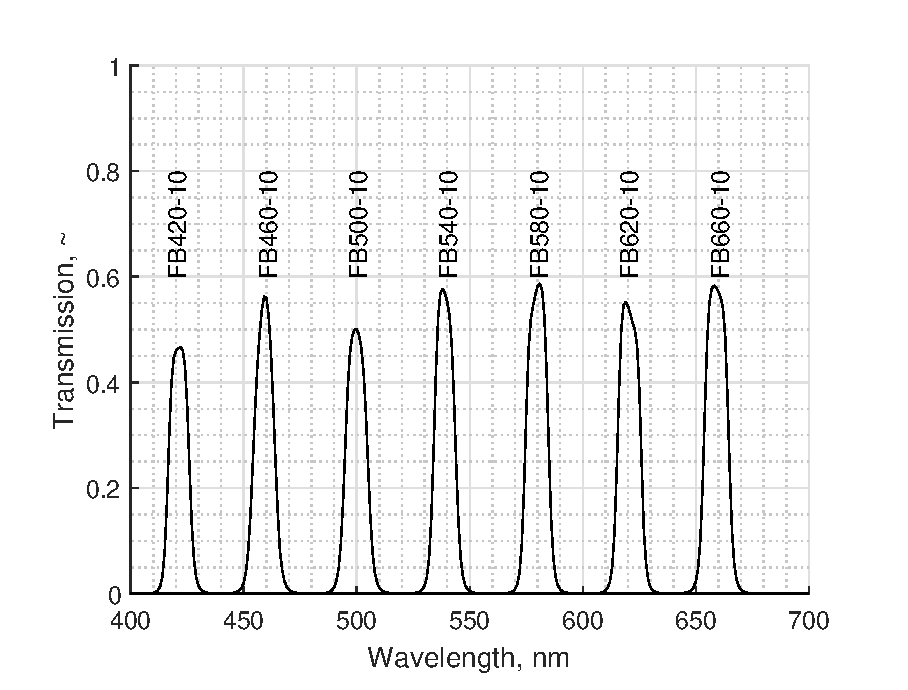
\includegraphics[width=0.5\textwidth]{thorlabs_filter_transmission_spectra.eps}
\caption{Thorlabs narrow bandpass filter transmission spectra, per manufacturer's datasheets. \cite{Thorlabs}}
\label{thorlabs_filter_transmission_spectra}
\end{figure}

\subsection{Camera Response Linearity}
\label{Camera Sensor Linearity}

RAW values reported from cameras may be thought of as photonic measurements. A simple under-exposure experiment found that pure black (i.e.\ zero photons) corresponds to RAW = 2,048. In principle, over-exposure and saturation occur at the maximum value permitted by the bit depth: $2^{14}$ = 16,384. In practice, saturation was observed at values nearly as low as 12,000. Between these limits, response linearity was verified by photographing the ColorChecker chart under noon daylight while independently varying shutter duration and ISO. The trichromate mode of the \#19 white swatch was calculated for each photo as the measurement of interest.

\id These measurements are shown in Figure \ref{linearity_shutter_data}. For ideal linearity, the RAW value is proportional to the product of shutter duration and ISO, all else equal. Accordingly, an idealized RAW value can be calculated for each reported RAW value, by linearly scaling the product of shutter duration and ISO to the RAW value range of [2,048 12,000]. This relationship can be expressed as a set of transfer functions, shown in Figure \ref{linearity_shutter_curves}. The shape of these transfer functions indicates that the sensor has a linear response up to saturation as expected. Similarly, varying ISO with a constant shutter duration exhibited near-perfect linearity (f/22, ISO 100-12,800, 1/2,000 sec).

\begin{figure}
\centering
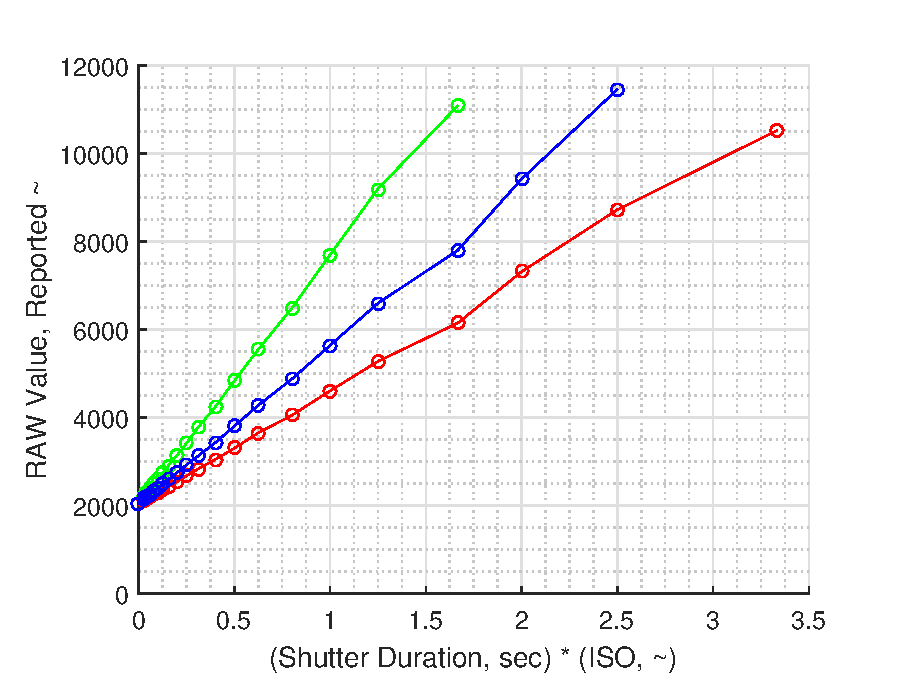
\includegraphics[width=0.5\textwidth]{linearity_shutter_data.eps}
\caption{Reported RAW values for \#19 white ColorChecker swatch in noon daylight without filters; f/22, ISO 100, 1/4,000-1/30 sec.}
\label{linearity_shutter_data}
\end{figure}

\begin{figure}
\centering
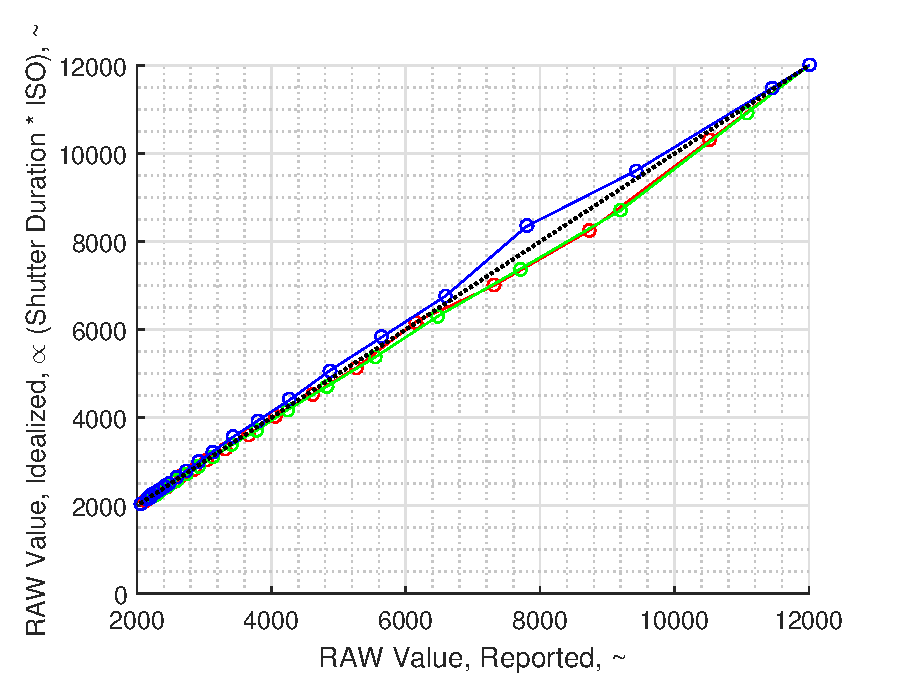
\includegraphics[width=0.5\textwidth]{linearity_shutter_curves.eps}
\caption{Photonic transfer functions for data in Figure \ref{linearity_shutter_data}.}
\label{linearity_shutter_curves}
\end{figure}

\subsection{Camera Spectral Sensitivity}
\label{Camera_Spectral_Sensitivity}

Camera spectral sensitivity is calculated by photographing a ColorChecker chart through each filter under cloudless noon daylight modeled as D65. Noon daylight was chosen for its roughly neutral SPD, availability of standard data, and accessibility. Images were captured on 2021-02-21 at 12:22 pm in an open field in Cambridge, Massachusetts. Each swatch produced a unique SPD modeled as the element-wise product of its spectral reflectance with the D65 illuminant. \cite{CVRL}

\id Reflectance spectra were measured using a Spectro 1 spectrophotometer with a domain of 400 to 700 nm and a resolution of 10 nm. Three scans were performed and averaged for each swatch, with near-perfect repeatability across trials. These spectra were validated by calculating the CIEDE2000 color difference (denoted $\Delta E_{00}$) against the manufacturer's published Lab color values under CIE D50 illuminant with a 2° observer. \cite{X-Rite} The error for all 24 swatches was 1.39 ± 1.06 $\Delta E_{00}$, showing good agreement. Research has shown significant variance in ColorChecker spectra, with standard deviations of 0.1-9.1 percentage points over 400-700 nm, though the manufacturer does not publish spectra or tolerances. \cite{BabelColor}

\id Assuming an ideal linear response as shown in Section \ref{Camera Sensor Linearity}, sensitivity may be described generally as:\\

$\mathrm{ Sensitivity = S = \dfrac{Value \ Measured}{Value \ Actual} } = \dfrac{V_M}{V_A}$ \\

$V_A = \mathlarger{\sum_{\lambda}} I(\lambda) \odot R(\lambda) \odot T(\lambda)$ \\

with: \\

\begin{tabular}{l | l}
$\lambda$ & Wavelength \\
I & Scene illuminant\\
R & Swatch reflectance \\
T & Filter transmission \\
$\odot$ & Element-wise multiplication \\
\end{tabular} \\

$V_M$ is calculated as the mode of the RAW values inside a square inset slightly from the swatch perimeter. Mode was chosen for its robustness against hot/dead pixels.

\id Sensitivity for all color channels and wavelengths can be calculated from any single swatch, as shown in Figure \ref{canon_650d_sensitivity}. These per-swatch sensitivity curves are fused as a weighted average using $V_M$. This has the effect of weighting calculated sensitivities in proportion to their signal-to-noise ratio.

\id The final result is a set of three sensitivity curves, $\left[ S_R(\lambda), \ S_G(\lambda), \ S_B(\lambda) \right]$. As shown in Figure \ref{camera_spectral_sensitivities}, this result is consistent with values from literature for similar Canon cameras.

\begin{figure}
\centering
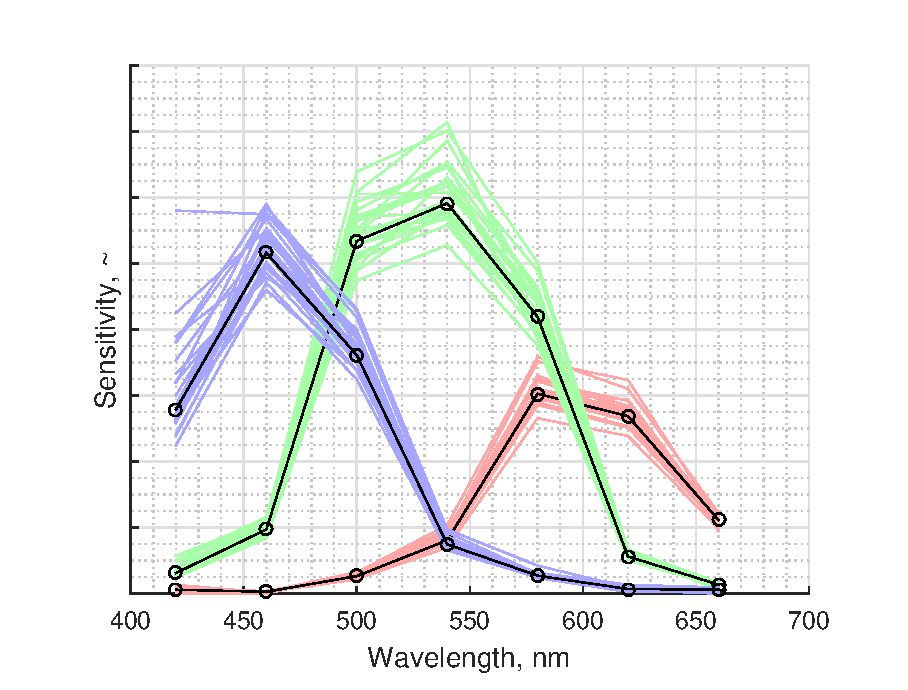
\includegraphics[width=0.5\textwidth]{canon_650d_sensitivity.eps}
\caption{Non-dimensional trichromate spectral sensitivity of Canon 650D camera from ColorChecker under D65 illuminant. Faint colored lines correspond to individual swatches; solid black lines correspond to weighted averages for all swatches.}
\label{canon_650d_sensitivity}
\end{figure}

\begin{figure}
\centering
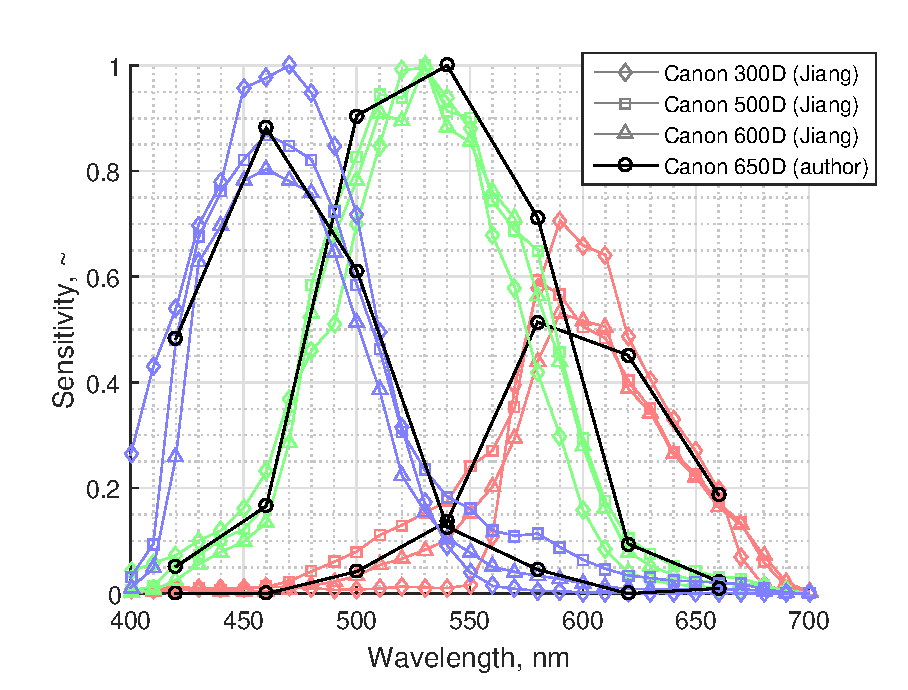
\includegraphics[width=0.5\textwidth]{camera_spectral_sensitivities.eps}
\caption{Comparison of normalized sensitivities for various Canon cameras. \cite{Jiang} Curves are normalized so that the maximum sensitivity for each camera is equal to unity.}
\label{camera_spectral_sensitivities}
\end{figure}

\subsection{Photographic Aspects}
\label{photographic}

A prime lens, tripod, quick release plate, and remote shutter are used to minimize movement of the camera while capturing the photo stack. Because filter cost is proportional to filter area, the choice of lens is the primary means of cost reduction. The measurement of interest is the diameter of the objective at the outer end of the lens, as it sets the minimum filter diameter. For consumer Canon EF lenses, this ranges from approximately 20 to 60 mm. The theoretical filter cost at these extremes differs by nearly an order of magnitude; $60^2 / 20^2 = 9$. The lens selected has an outer objective diameter of 20 mm, a focal length of 40 mm, and an aperture of f/2.8. It is shown in Figure \ref{canon}.

\id The filters discussed in Section \ref{section_filters} are unthreaded, and used by resting them against the camera lens by hand, transferring minimal force and maintaining alignment of the photo stack. The lens and filters are designed such that their glass optics are recessed from their cases. The filters are stored in a case in order of ascending wavelength, and cycled through in sequence manually.

\id Depending on the nature and luminance of the scene, typical camera settings are f/2.8-10, ISO 100-400, and 1/4 - 1/500 second. Bright exposures are required to compensate for the low transmission of the filters. These settings are collectively adjusted to ``expose to the right'', i.e.\ fully utilize the available set of values without saturating the upper limit, thereby maximizing the signal-to-noise ratio in the measured values.

\begin{figure}
\centering
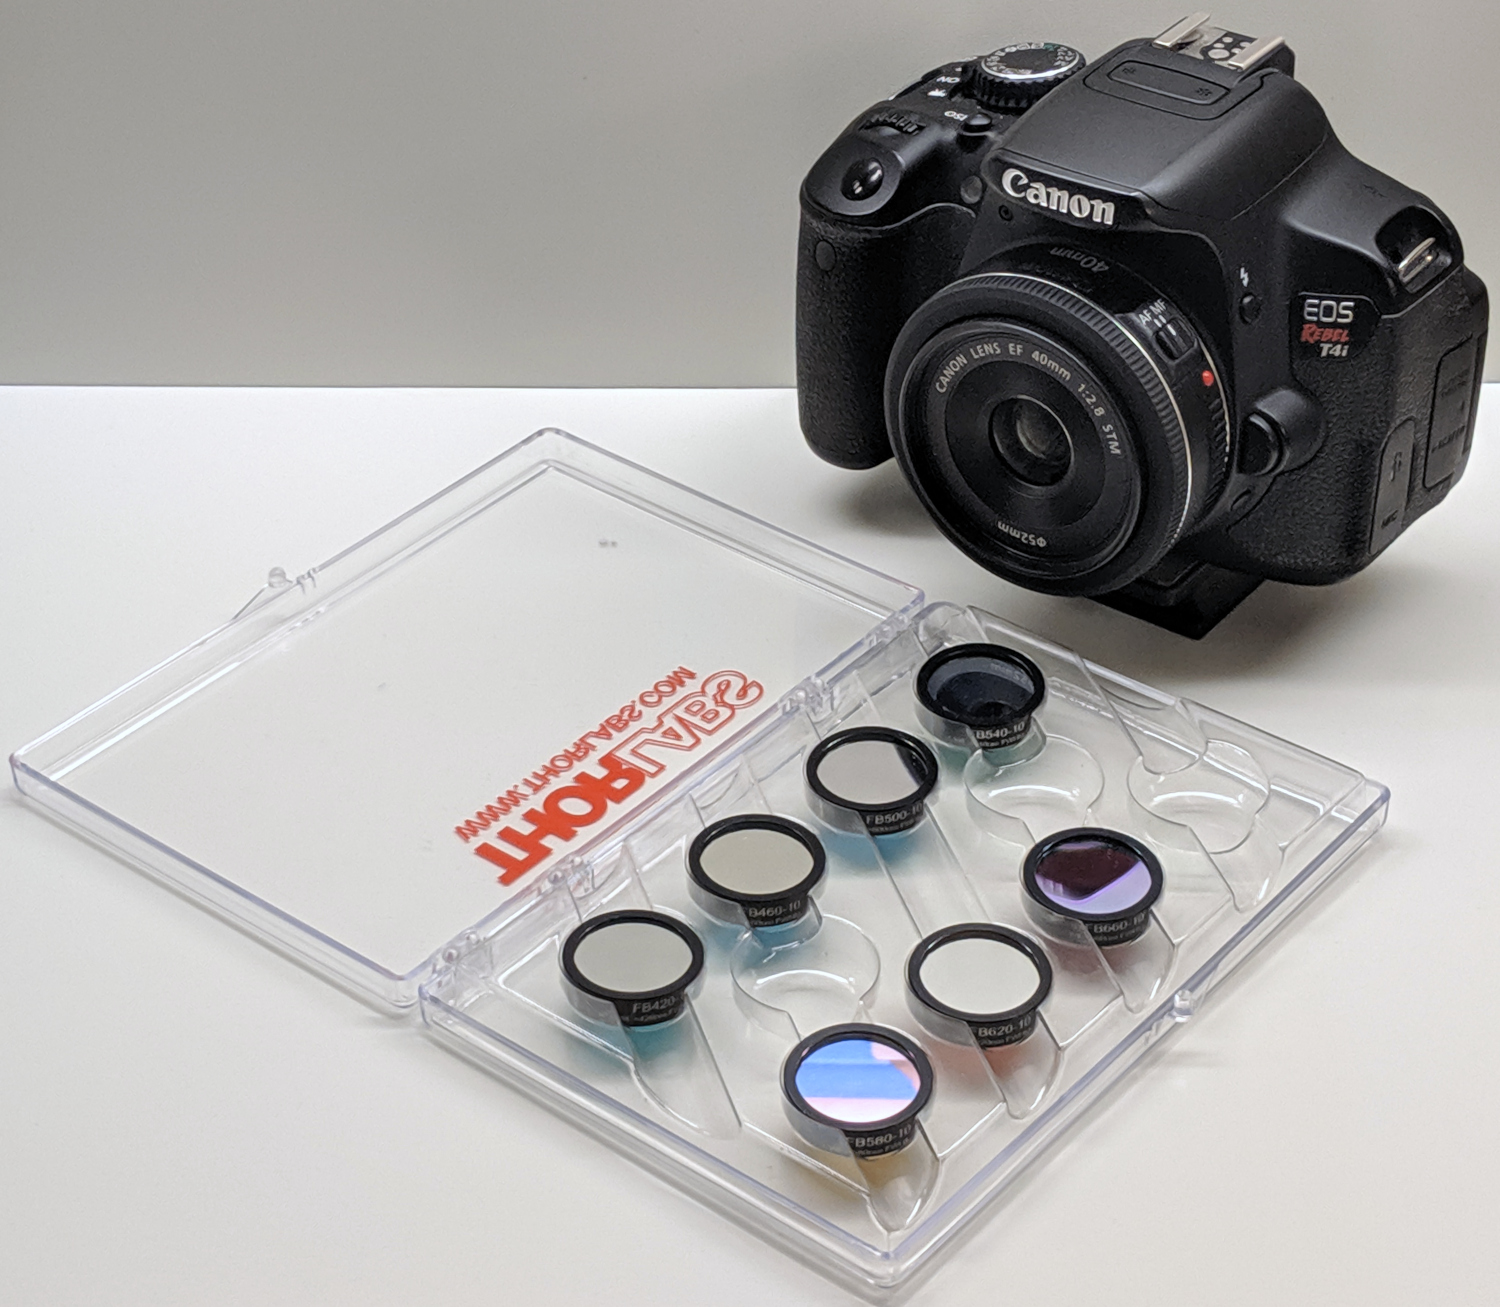
\includegraphics[width=0.45\textwidth]{IMG_20210712_212507_GIMP.jpg}
\caption{Canon 650D camera with 40 mm prime EF lens, and set of Thorlabs narrow bandpass filters.}
\label{canon}
\end{figure}

\id The open-source \texttt{dcraw} utility is used to extract RAW values stored in the .CR2 file format. \cite{dcraw} The modifier string \texttt{-D -4 -j -t 0} specifies that the extracted RAW values are unprocessed sensor measurements:\\

\begin{tabular}{l | l}
-D & No value scaling \\
-4 & Linear 16-bit \\
-j & No stretching or rotating pixels \\
-t 0 & No image rotation \\
\end{tabular} \\

The RAW sensor measurements are then demosaiced into R, G, B color channels with a Bayer filter pattern of \texttt{rggb}.

\subsection{SPDs from RAW Photos}

 By rearranging the general expression of sensitivity in Section \ref{Camera_Spectral_Sensitivity}: \\

 $V_A = \dfrac{V_M}{S}$ \\

For a linear sensor response, $V_M \propto P$, with $P$ denoting the RAW photo value. By inspection, $V_A \propto SPD$. Using proportionality and non-dimensionality, this is rearranged and substituted as: \\

 $SPD = V_A = \dfrac{P}{ST}$ \\

Filter transmission $T$ is accounted for as a factor acting on $S$, a property of the camera only. The denominator $ST$ is most accurately and generally expressed as $S(\lambda) \cdot T(\lambda)$, rather than $S(\lambda=CWL) T(\lambda=CWL)$, i.e.\ a dot product over the wavelength domain, rather than a scalar product at the CWL.

\id At an arbitrary pixel and CWL, each color channel produces an independent SPD measurement, collectively given as: \\

 $SPD = \left[ \dfrac{P_R}{S_R \cdot T},\dfrac{P_G}{S_G \cdot T},\dfrac{P_B}{S_B \cdot T} \right] $ \\

These measurements are theoretically equal, but in practice differ as a result of various sources of error. They are fused as a sensitivity-weighted average: \\

$\overline{SPD} = \dfrac{1}{S_R+S_G+S_B} \left( \dfrac{P_R S_R}{S_R \cdot T} + \dfrac{P_G S_G}{S_G \cdot T} + \dfrac{P_B S_B}{S_B \cdot T} \right)$\\

Calculating $\overline{SPD}$ as a sensitivity-weighted average continuously interpolates between color channels as a function of wavelength. Since $S_R+S_G+S_B > 0$ for all $\lambda$, divide-by-zero is precluded. This formulation generalizes spatially by using matrices in place of scalars for $P$, neglecting vignetting, dark-frame effects, and other spatially-related sources of error.

\id The HSDC is first calculated in a sparse fashion, only at the CWLs of the filters. The full (i.e.\ non-sparse) HSDC is then calculated by cubic interpolation in the wavelength domain between the filter CWLs per Section \ref{curve_reconstruction}.

\section{Results}
\subsection{Validation}
\label{validation}

The method is validated by comparing ColorChecker SPDs and $\Delta E_{00}$ between camera vs.\ spectrophotometer, with the latter taken as ground truth and modeled as $R(\lambda) \odot I(\lambda)$. Because the two sets of curves, $SPD_{camera}$ and $SPD_{spectrophotometer}$, are non-dimensional, their ranges are aligned with a single scalar gain for comparative purposes, such that the sum of the residuals is zero. This scalar gain $\alpha$ is found by the bisection method such that:\\

$\mathlarger{ \sum_{\lambda}} ( \alpha SPD_{camera}- SPD_{spectrophotometer} )=0$ \\

Standard equations are used to derive XYZ, Lab, and RGB colors from SPDs, with D65 as both the scaling factor and white point. \cite{Lindbloom}

%
%$X = \dfrac{1}{N} \mathlarger{ \sum_{\lambda}} \hspace{1 mm} \bar{x} \odot SPD(\lambda) \Delta \lambda$\\
%$Y = \dfrac{1}{N} \mathlarger{ \sum_{\lambda}} \hspace{1 mm} \bar{y} \odot SPD(\lambda) \Delta \lambda$\\
%$Z = \dfrac{1}{N} \mathlarger{ \sum_{\lambda}} \hspace{1 mm} \bar{z} \odot SPD(\lambda) \Delta \lambda$\\
%$N = \mathlarger{ \sum_{\lambda}} \hspace{1 mm} \bar{y} \odot I(\lambda) \Delta \lambda$\\
%
%The specific formulation for $SPD(\lambda)$ is given by:\\
%
%\begin{tabular}{l l l}
%$SPD_{camera}$ & $= SPD(\lambda)$ & (Emissive case) \\
%$SPD_{spectrophotometer}$ & $= R(\lambda) \odot I(\lambda)$ & (Reflective case) \\
%\end{tabular}\\

\id Results are shown in Figures \ref{colorchecker} and \ref{colorchecker_SPDs}. The color error for all swatches is 2.44 $\pm$ 1.65 $\Delta E_{00}$, with more than 90\% of swatches within 1.75 $\pm$ 0.96 $\Delta E_{00}$ . The primary outlier is \#19 white, which shows a good match in terms of normalized distribution, but a poor match in magnitude and thus luminance. This is best explained as an artifact of glare or other lighting non-uniformities, amplified by the high reflectance of the color white. Corroborating this, the SPDs of the matte black background show a spatial luminance variance that matches the SPD magnitude error.

\id In the more general case of an unknown illuminant, colors are dimensionalized by linear scaling in the luminance (or intensity) dimension to the limits of the color space. Scaling based on minimum and maximum values is inadvisable due to the possible presence of hot/dead pixels. A common robust strategy is allow a small amount of saturation at the limits of the color space. Reconstructed images in this paper are scaled such that the bottom and top 1\% of pixels are saturated, with black and white defined as 5\% and 95\% (i.e. RGB [13,13,13], [242,242,242]) respectively.

%luminance CDF may be calculated and scaled such that the image fully utilizes the color space's luminance range with negligible saturation at both extreme ends. This is stated using typical values as:\\
%
%\begin{tabular}{l l}
%Luminance(CDF = 1\%) & = 5\%\\
%Luminance(CDF = 99\%) & = 95\%\\
%\end{tabular}\\

%\subsection{Images from HSDCs}

\clearpage

\onecolumn

\begin{table}[H]
\centering
\begin{tabular}{cc}
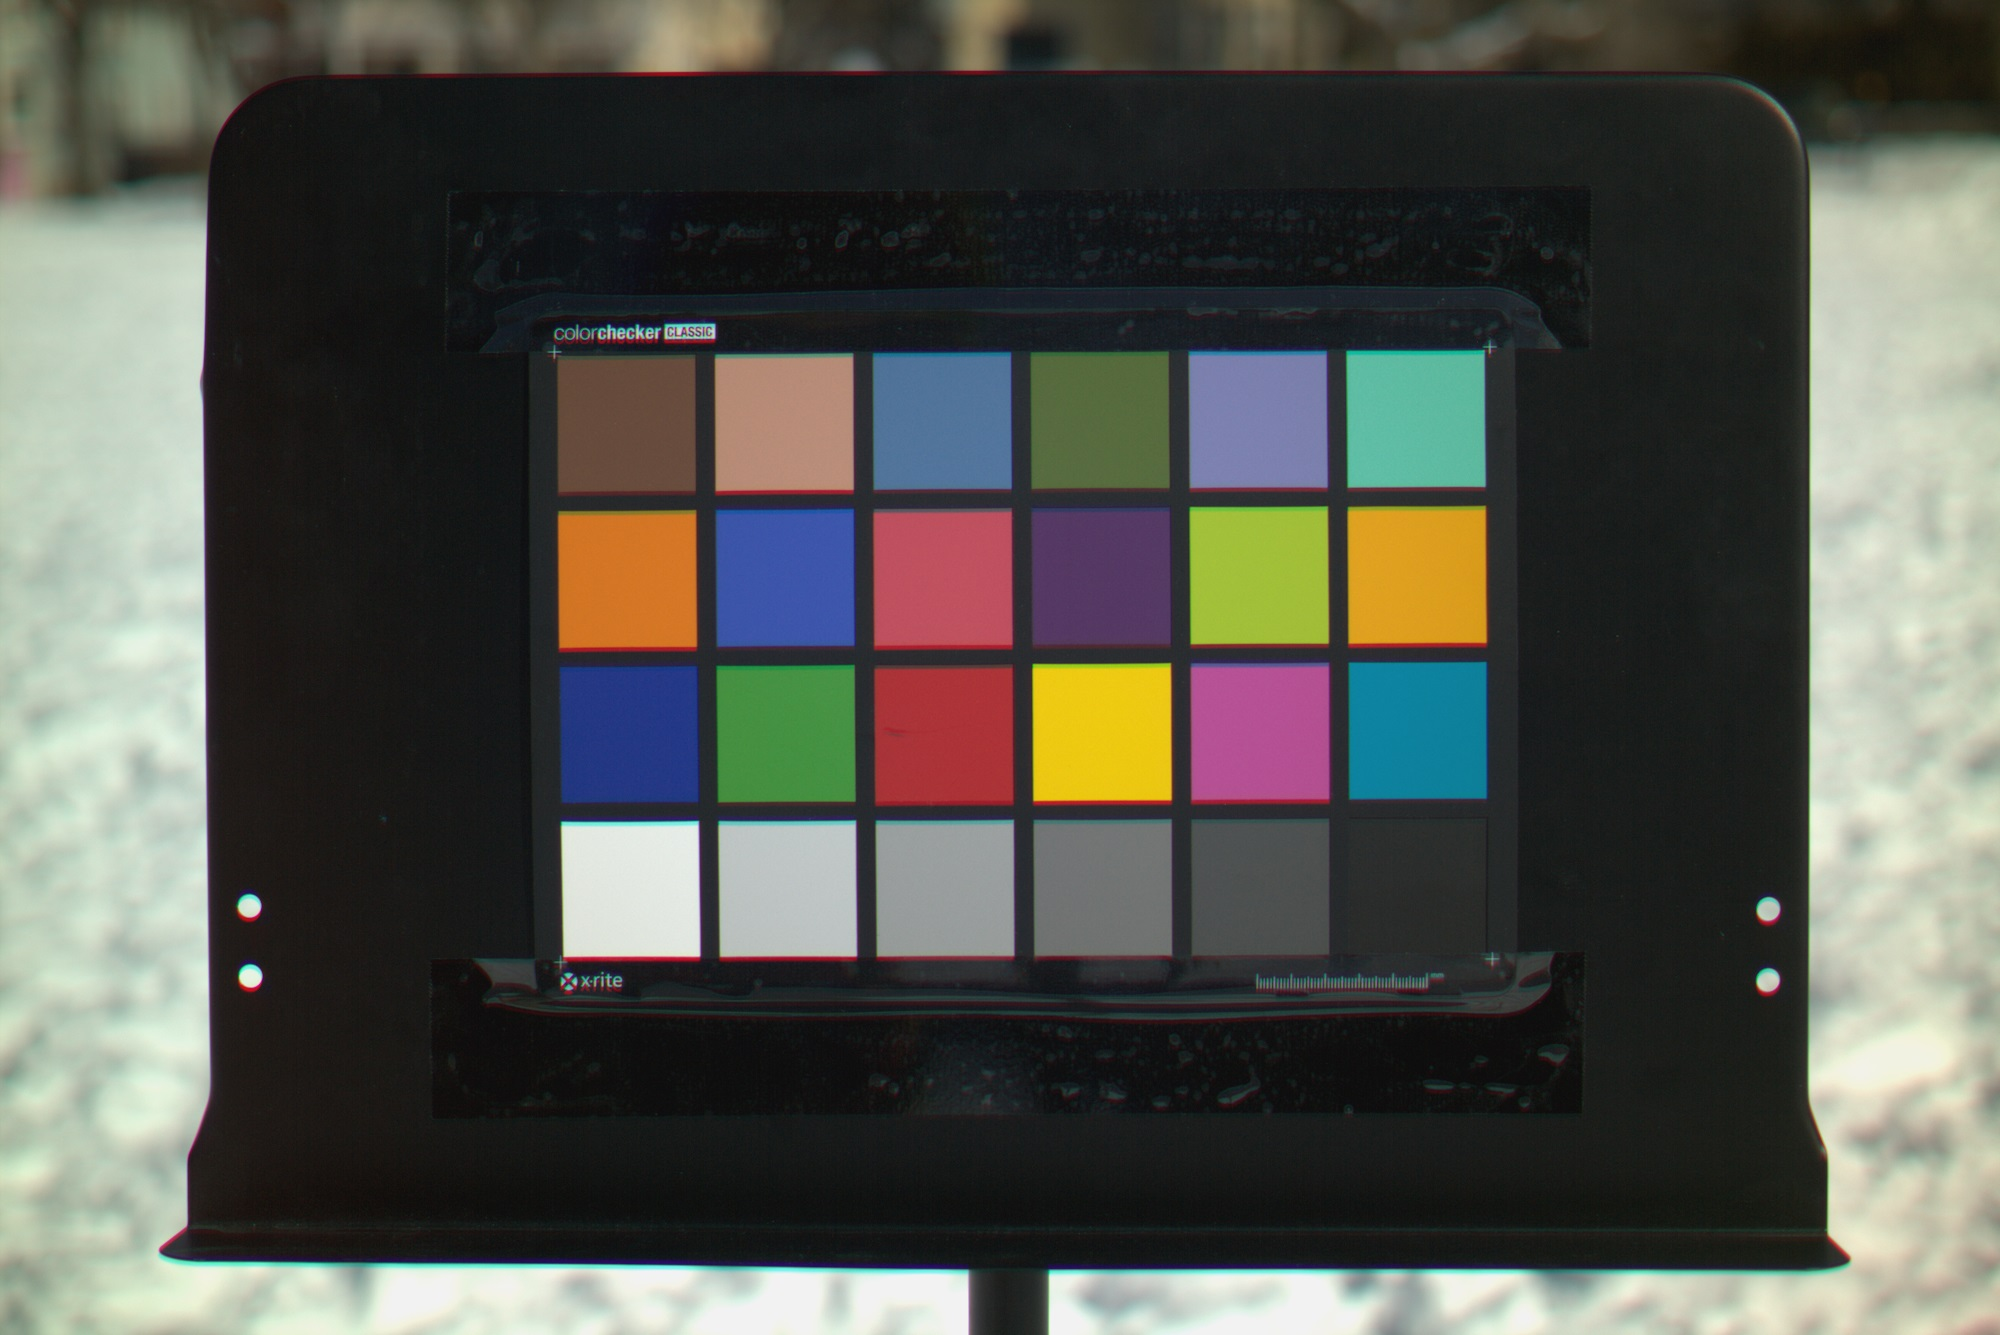
\includegraphics[width=0.45\linewidth]{colorchecker.jpg} & 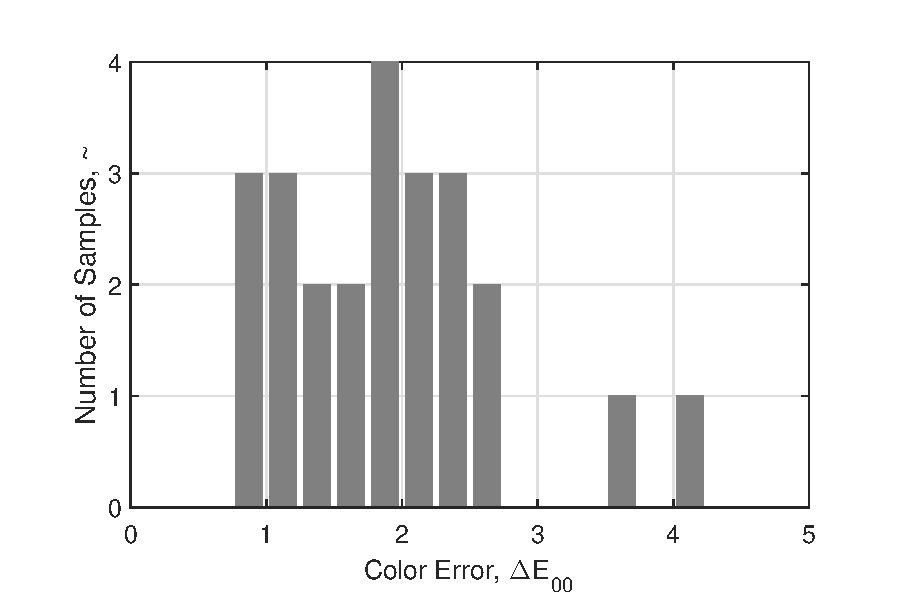
\includegraphics[width=0.45\linewidth]{error_summary.eps} \\
\end{tabular}
\captionof{figure}{Left: reconstructed image of ColorChecker chart; f/2.8, ISO 100, 1/400 sec. Right: distribution of color errors shown in Figure \ref{colorchecker_SPDs}.}
\label{colorchecker}
\end{table}

%\begin{figure}[H]
%\begin{centering}
%  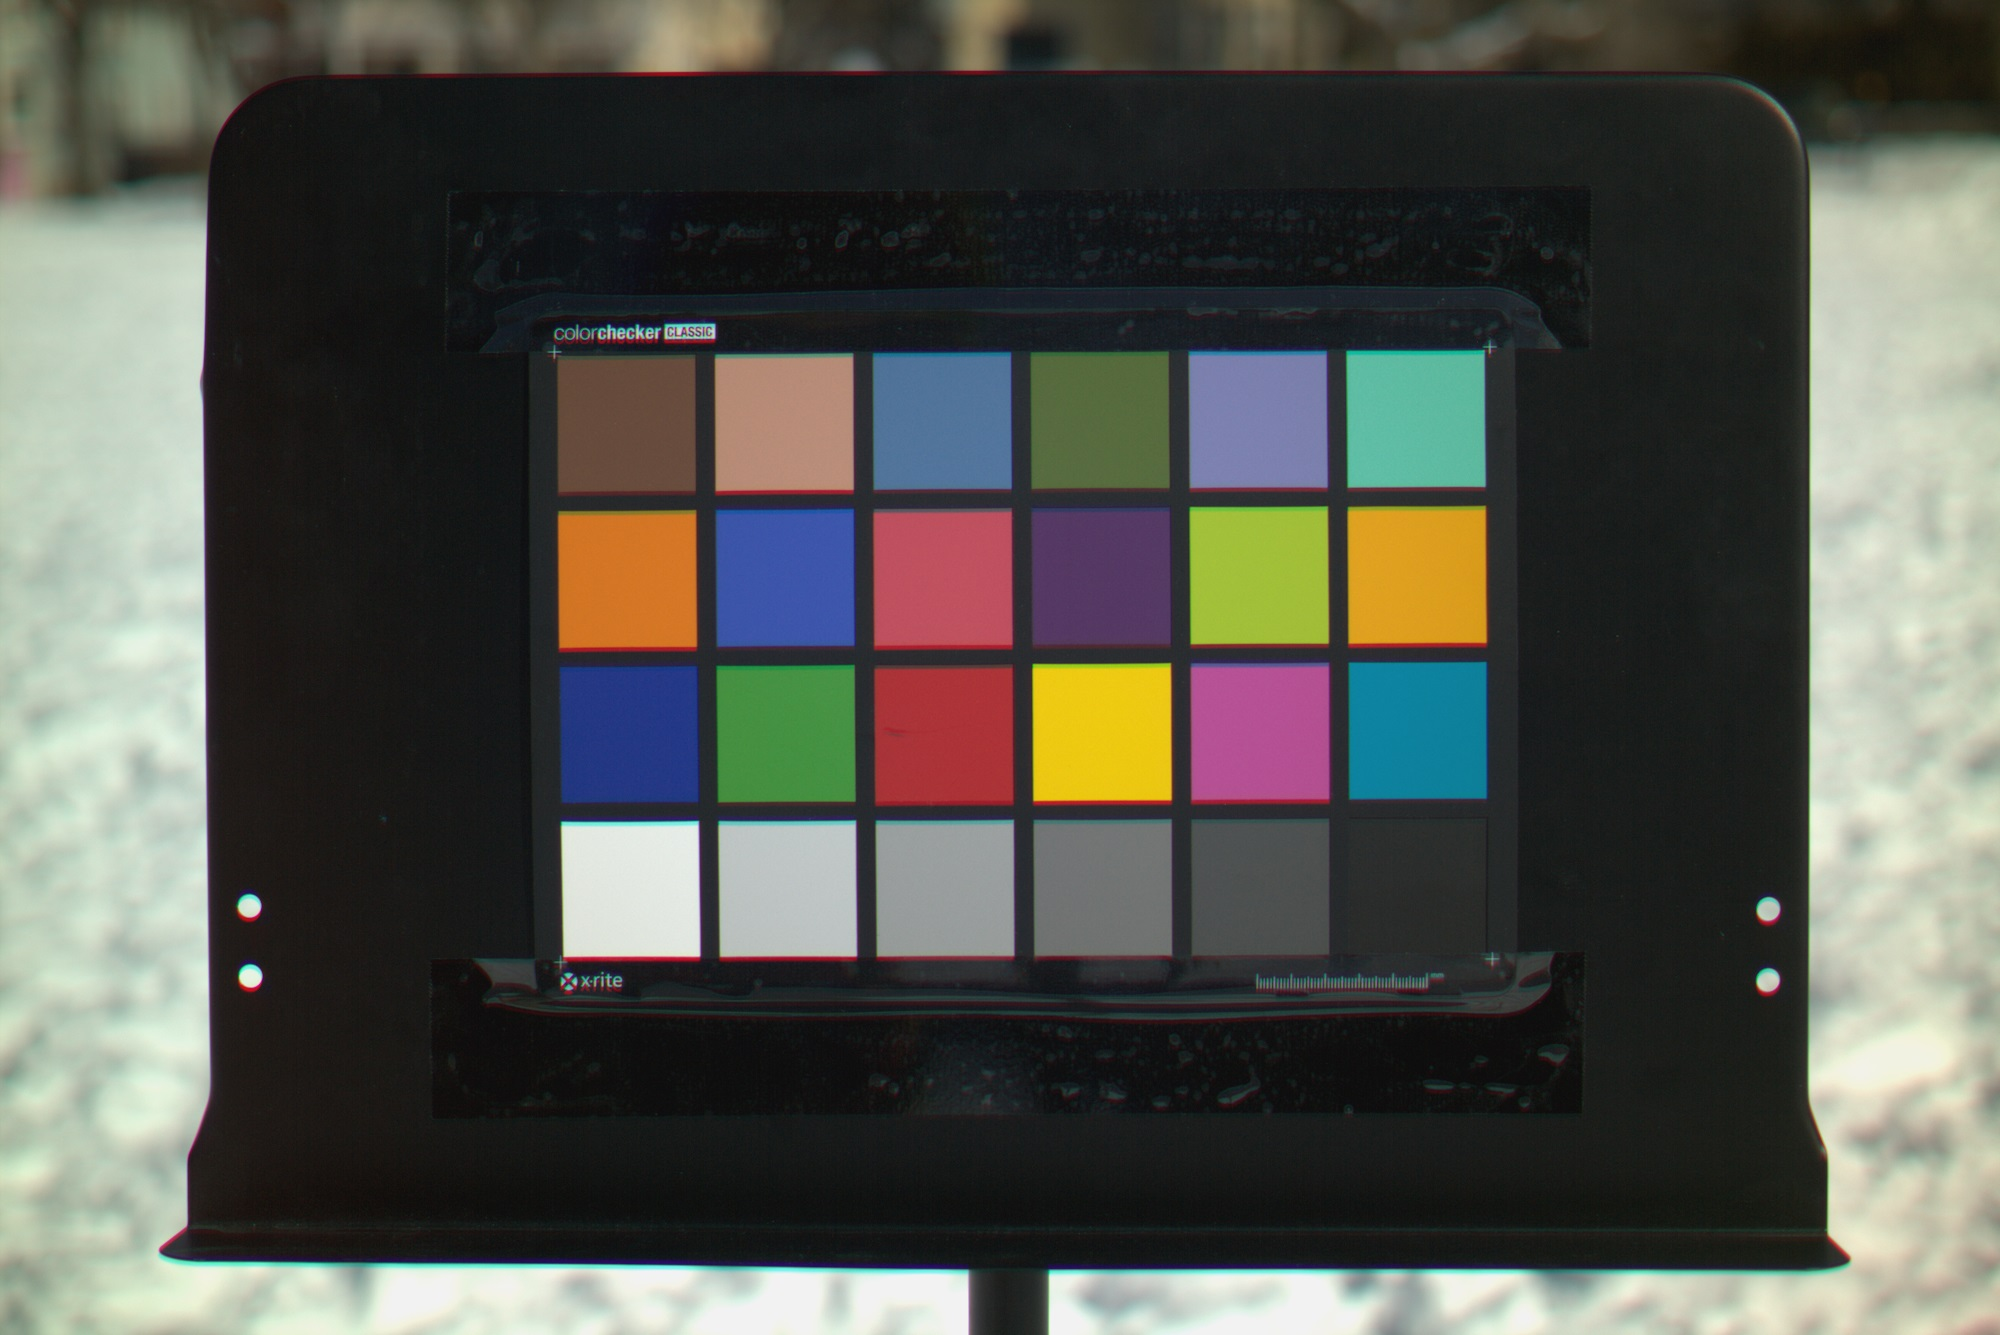
\includegraphics[height=0.25\linewidth]{colorchecker.jpg}
%  \caption{Reconstructed image of ColorChecker chart under noon daylight; f/2.8, ISO 100, 1/400 sec.}
%  \label{colorchecker_mesh}
%  \end{centering}
%\end{figure}

\begin{figure}[H]
\begin{centering}
  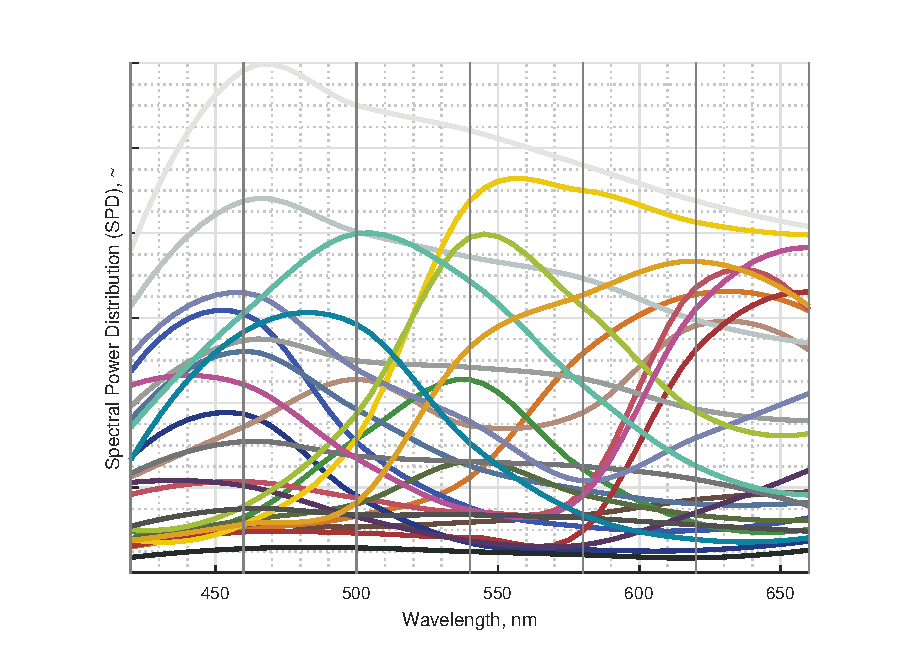
\includegraphics[height=0.60\linewidth]{colorchecker_SPDs.eps}
    \caption{Comparison of SPDs and colors as measured by spectrophotometer (solid, left) and camera (dashed, right). A single scalar gain is applied to align the magnitudes of the two sets of curves. $\Delta E_{00}$ is reported for each swatch. Plots are scaled 400 to 700 nm along x, and non-dimensional along y.}
  \label{colorchecker_SPDs}
    \end{centering}
\end{figure}


%\begin{figure}[H]
%\begin{centering}
%  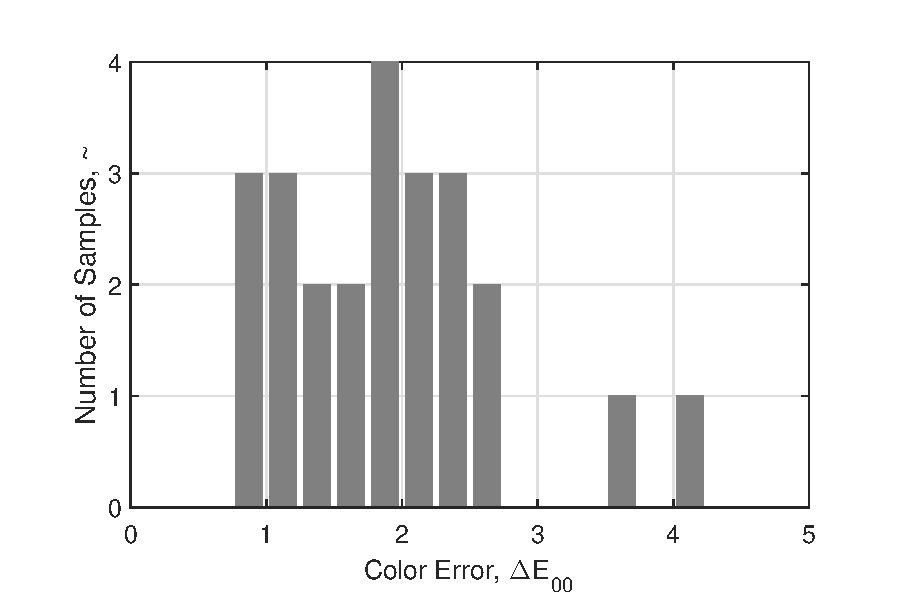
\includegraphics[height=0.10\linewidth]{error_summary.eps}
%    \caption{Distribution of color errors shown in Figure \ref{colorchecker_SPDs}.}
%  \label{error_summary}
%    \end{centering}
%\end{figure}

\clearpage
%\twocolumn

\subsection{Reconstructed Images}

%\onecolumn

Several scenes are shown in Figure \ref{reconstructed_images} with subjects and illuminants that represent typical color perception. Shown for each scene is the reconstructed image (left column) and a sparse sampling of the HSDC (right column). Each HSDC is sampled at an evenly-distributed 10 x 7 square mesh with 70 nodes total, showing a characteristic set of SPDs that are colored according the reconstructed image.

\id The still life (first row) exhibits blue-red contrast apparent in the bimodal distribution of the SPDs. A relatively high f-stop was needed to keep the scene in focus, which required increasing both ISO and shutter duration. The lower signal-to-noise ratio inherent with higher ISO can be seen in the high-frequency noise pattern. The camera settings were f/10, ISO 400, 1/4 second.

\id The landscape (second row) exhibits both color and luminance contrast between sky and ground. Modest ``spectral smearing'' can be seen around the edges of the foliage due to natural movement. The sky exhibits a characteristic D65-like distribution. Higher overall luminance enabled lower ISO and higher shutter duration, reducing noise. The camera settings were f/2.8, ISO 200, 1/200 second.

\id The industrial scene (third row) exhibits correlation between SPDs that is consistent with the yellow-red light characteristic of sunsets. The camera settings were f/4, ISO 200, 1/60 second.

\vfill

\begin{table}[H]
\centering
\begin{tabular}{cc}
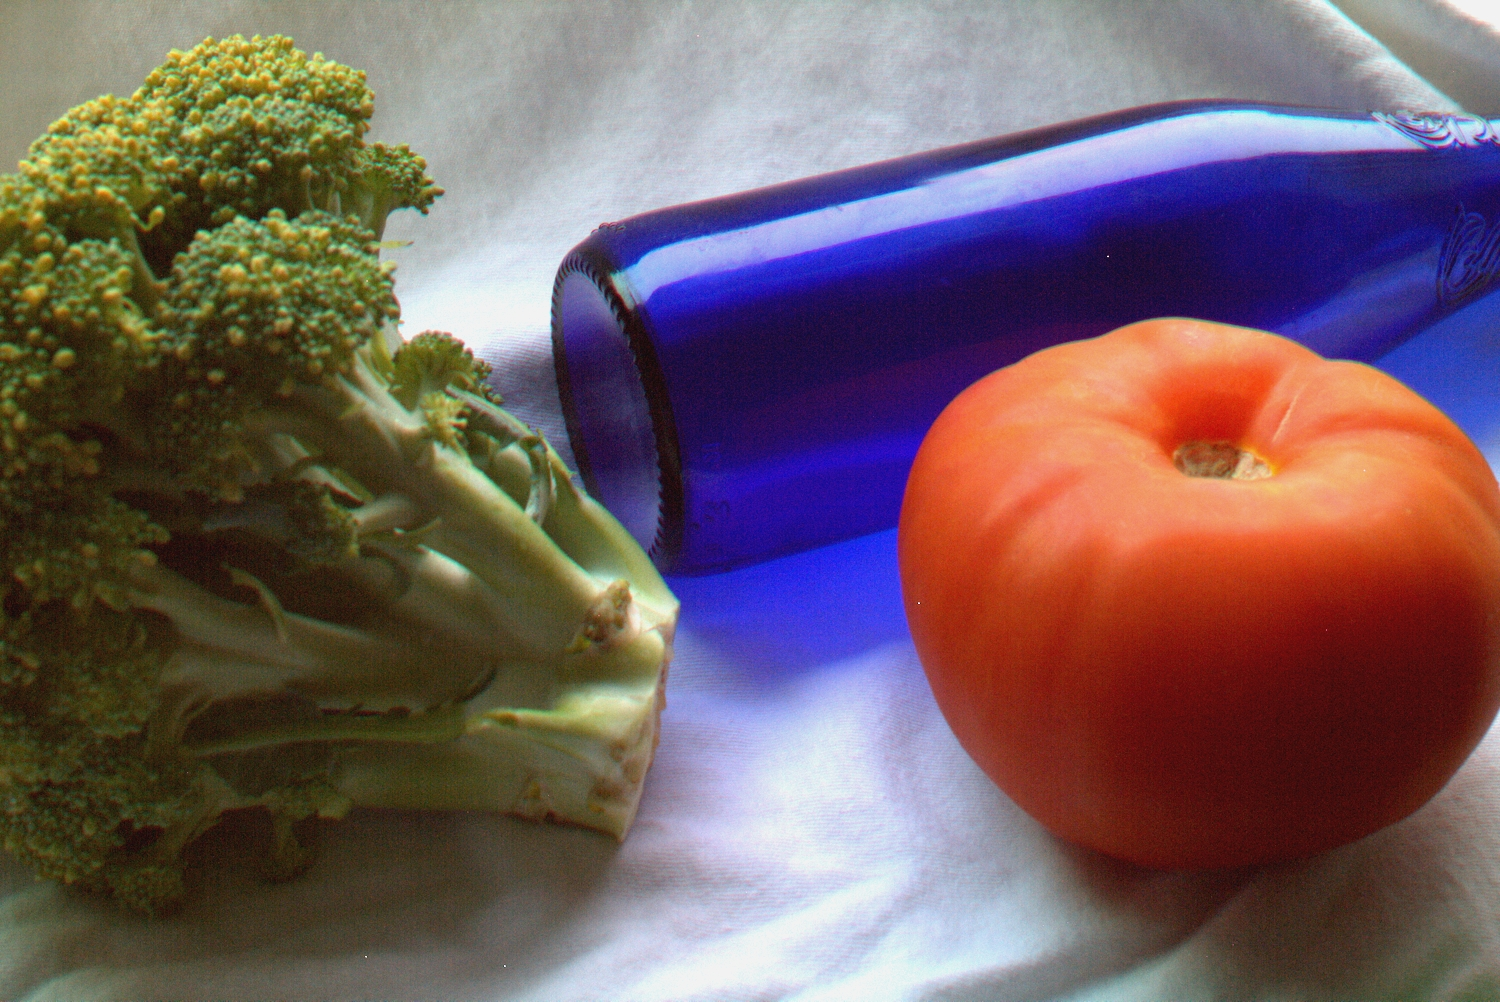
\includegraphics[width=0.40\linewidth]{IMG_4795_hyperspectral_1500_px_06-Aug-2021_14-12-44.jpg} & 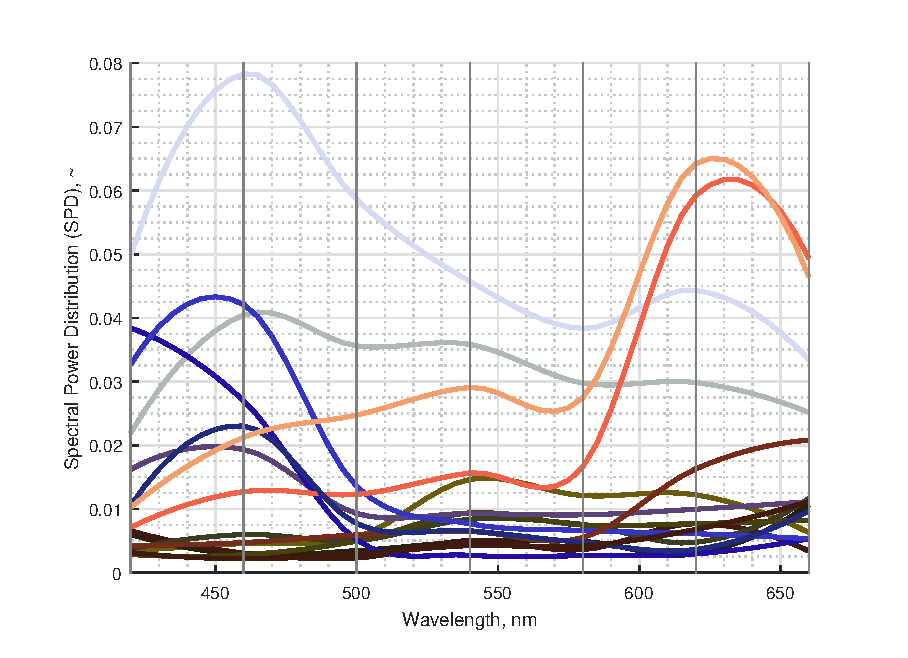
\includegraphics[width=0.40\linewidth]{broccoli_bottle_tomato.eps} \\
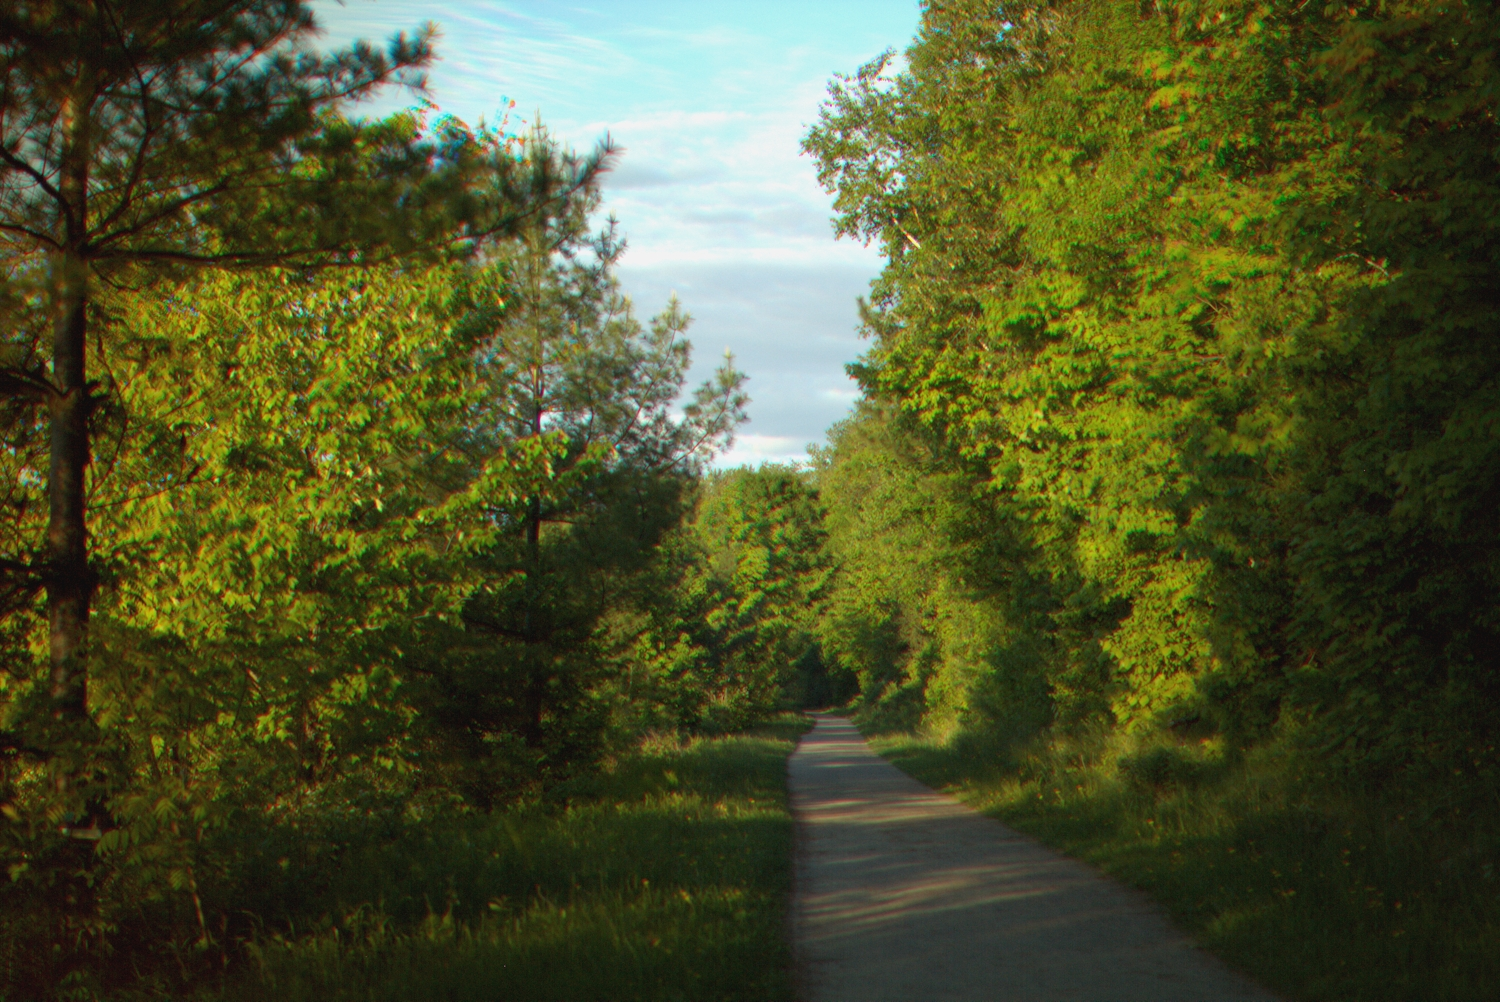
\includegraphics[width=0.40\linewidth]{IMG_4422_hyperspectral_1500_px_06-Aug-2021_14-14-50.jpg} & 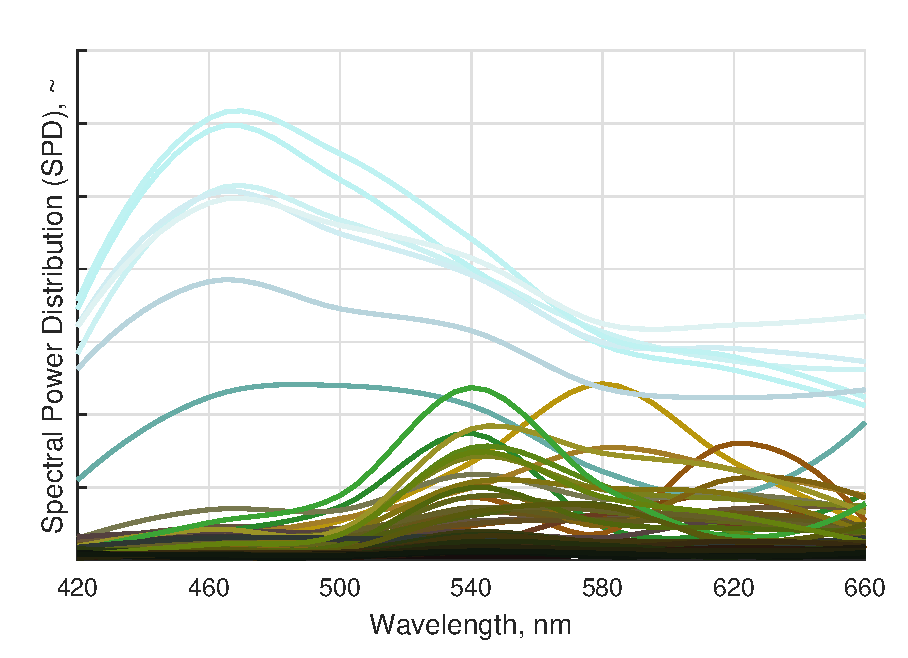
\includegraphics[width=0.40\linewidth]{vermont_path.eps} \\
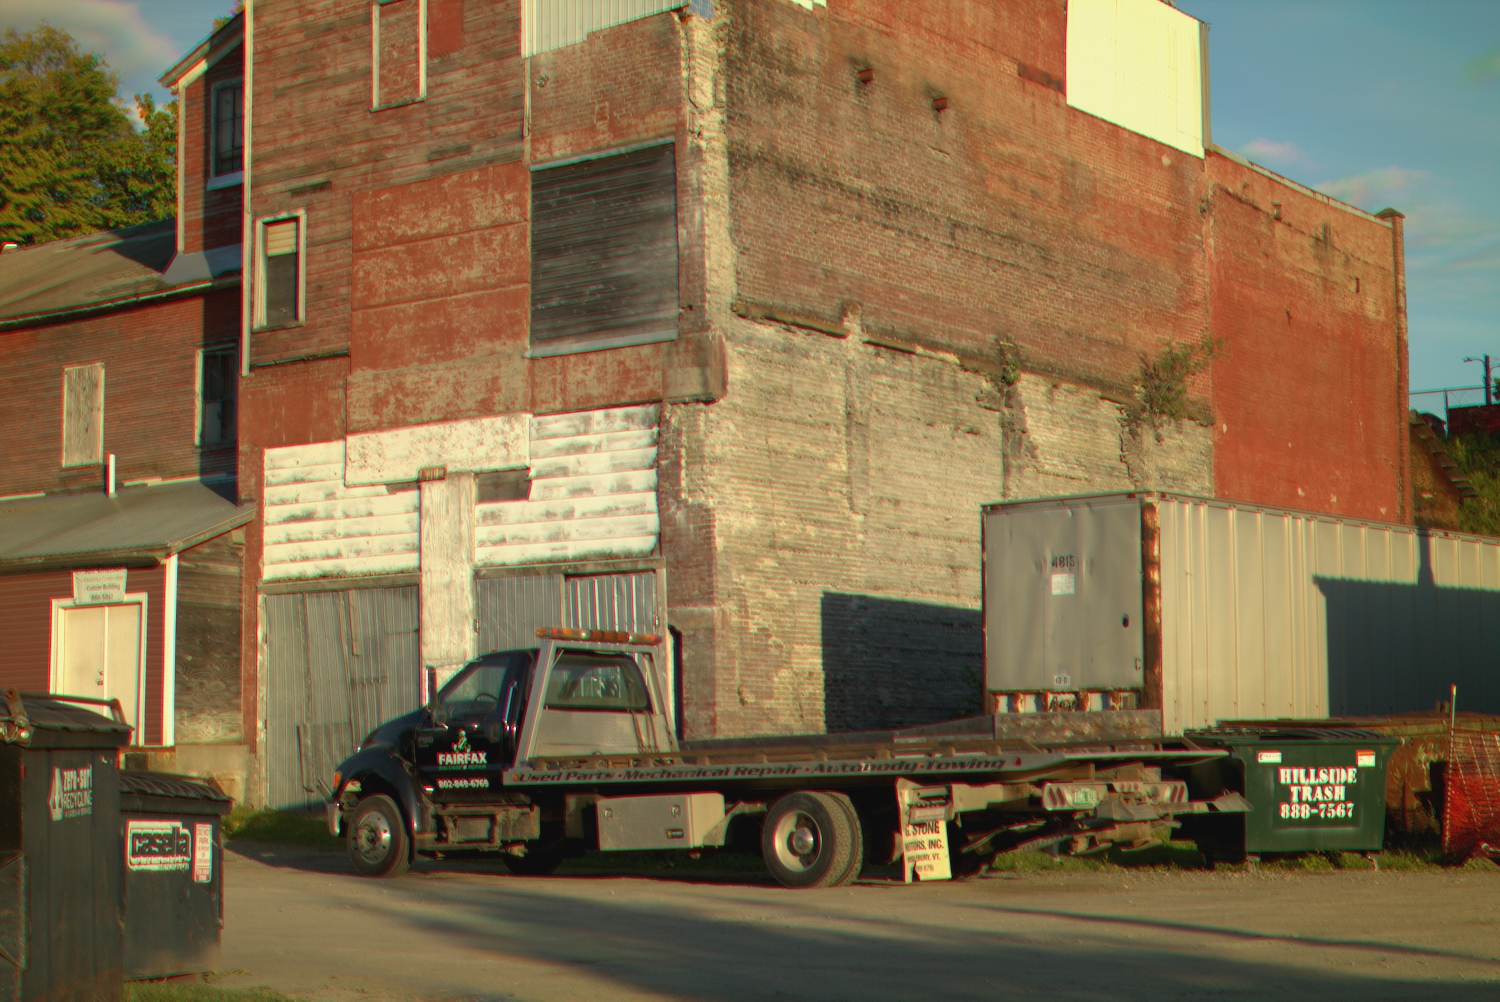
\includegraphics[width=0.40\linewidth]{IMG_4407_hyperspectral_1500_px_06-Aug-2021_14-08-54} & 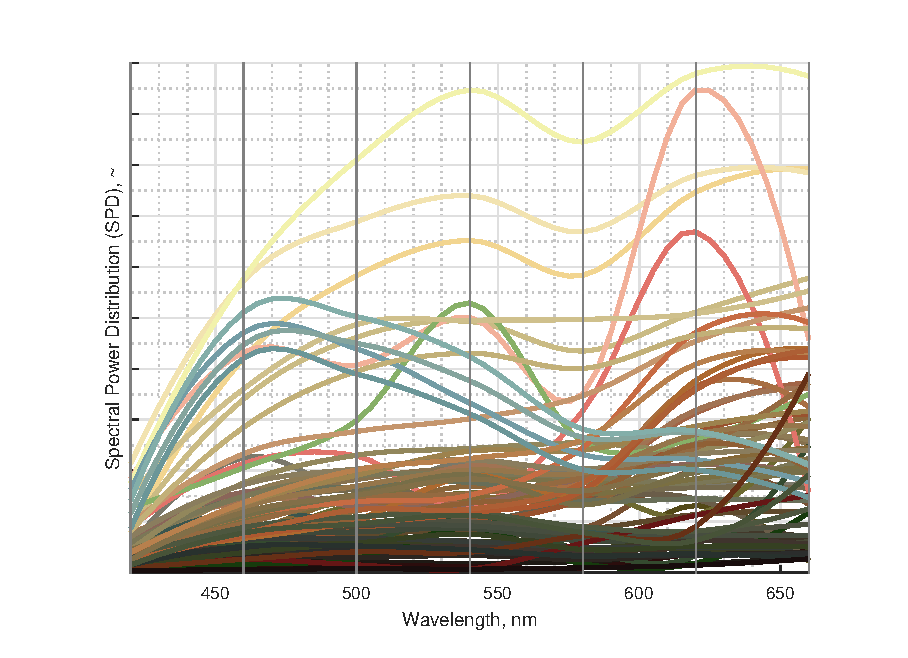
\includegraphics[width=0.40\linewidth]{truck_SPDs.eps} \\
\end{tabular}
\captionof{figure}{Reconstructed RGB images and characteristic sets of SPDs for several scenes.}
\label{reconstructed_images}
\end{table}

%\begin{figure}[H]
%\begin{centering}
%  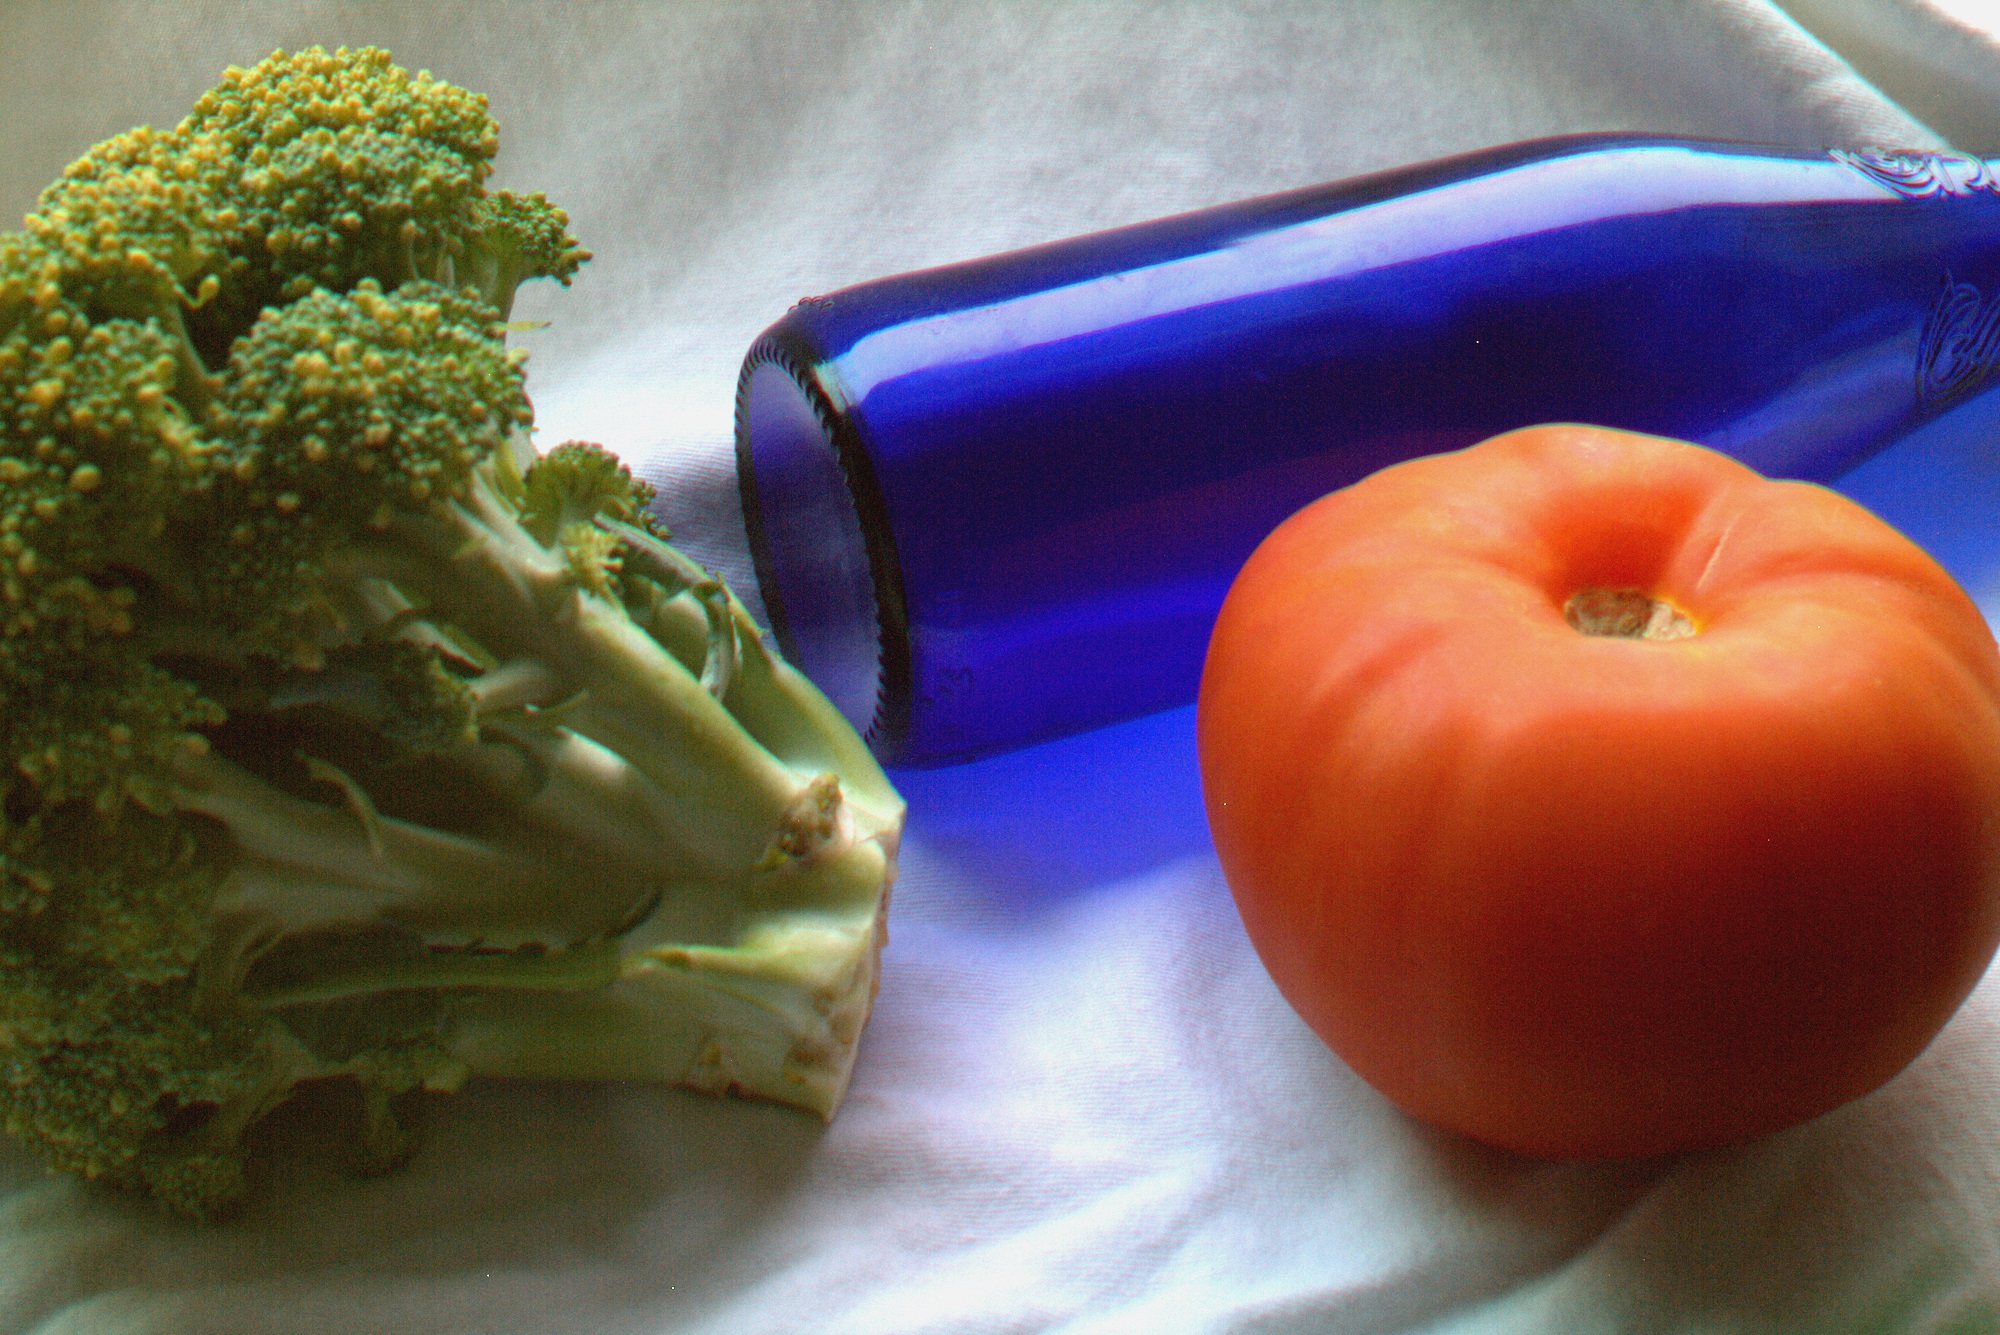
\includegraphics[width=0.30\linewidth]{broccoli_bottle_tomato.jpg}
%  \caption{Reconstructed image of still life under evening horizon light; f/10, ISO 400, 1/4 sec.}
%%  \label{tomato_mesh}
%  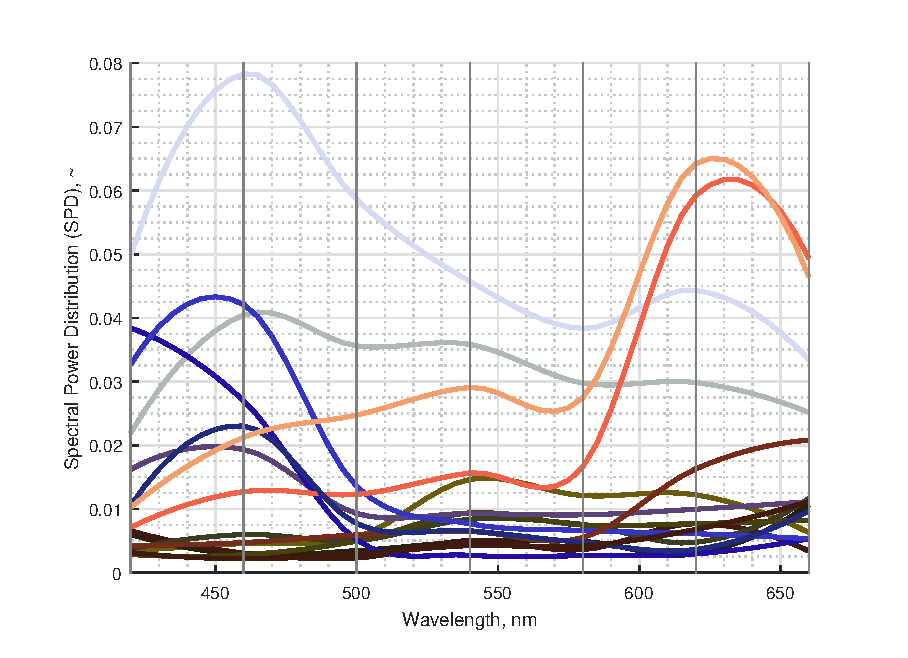
\includegraphics[width=0.30\linewidth]{broccoli_bottle_tomato.eps}
%  \caption{SPDs and reconstructed colors sampled at a 70-node square mesh for the scene in Figure \ref{tomato_mesh}.}
%  \label{tomato_SPDs}
%  \end{centering}
%\end{figure}
%
%\begin{figure}[H]
%\begin{centering}
%  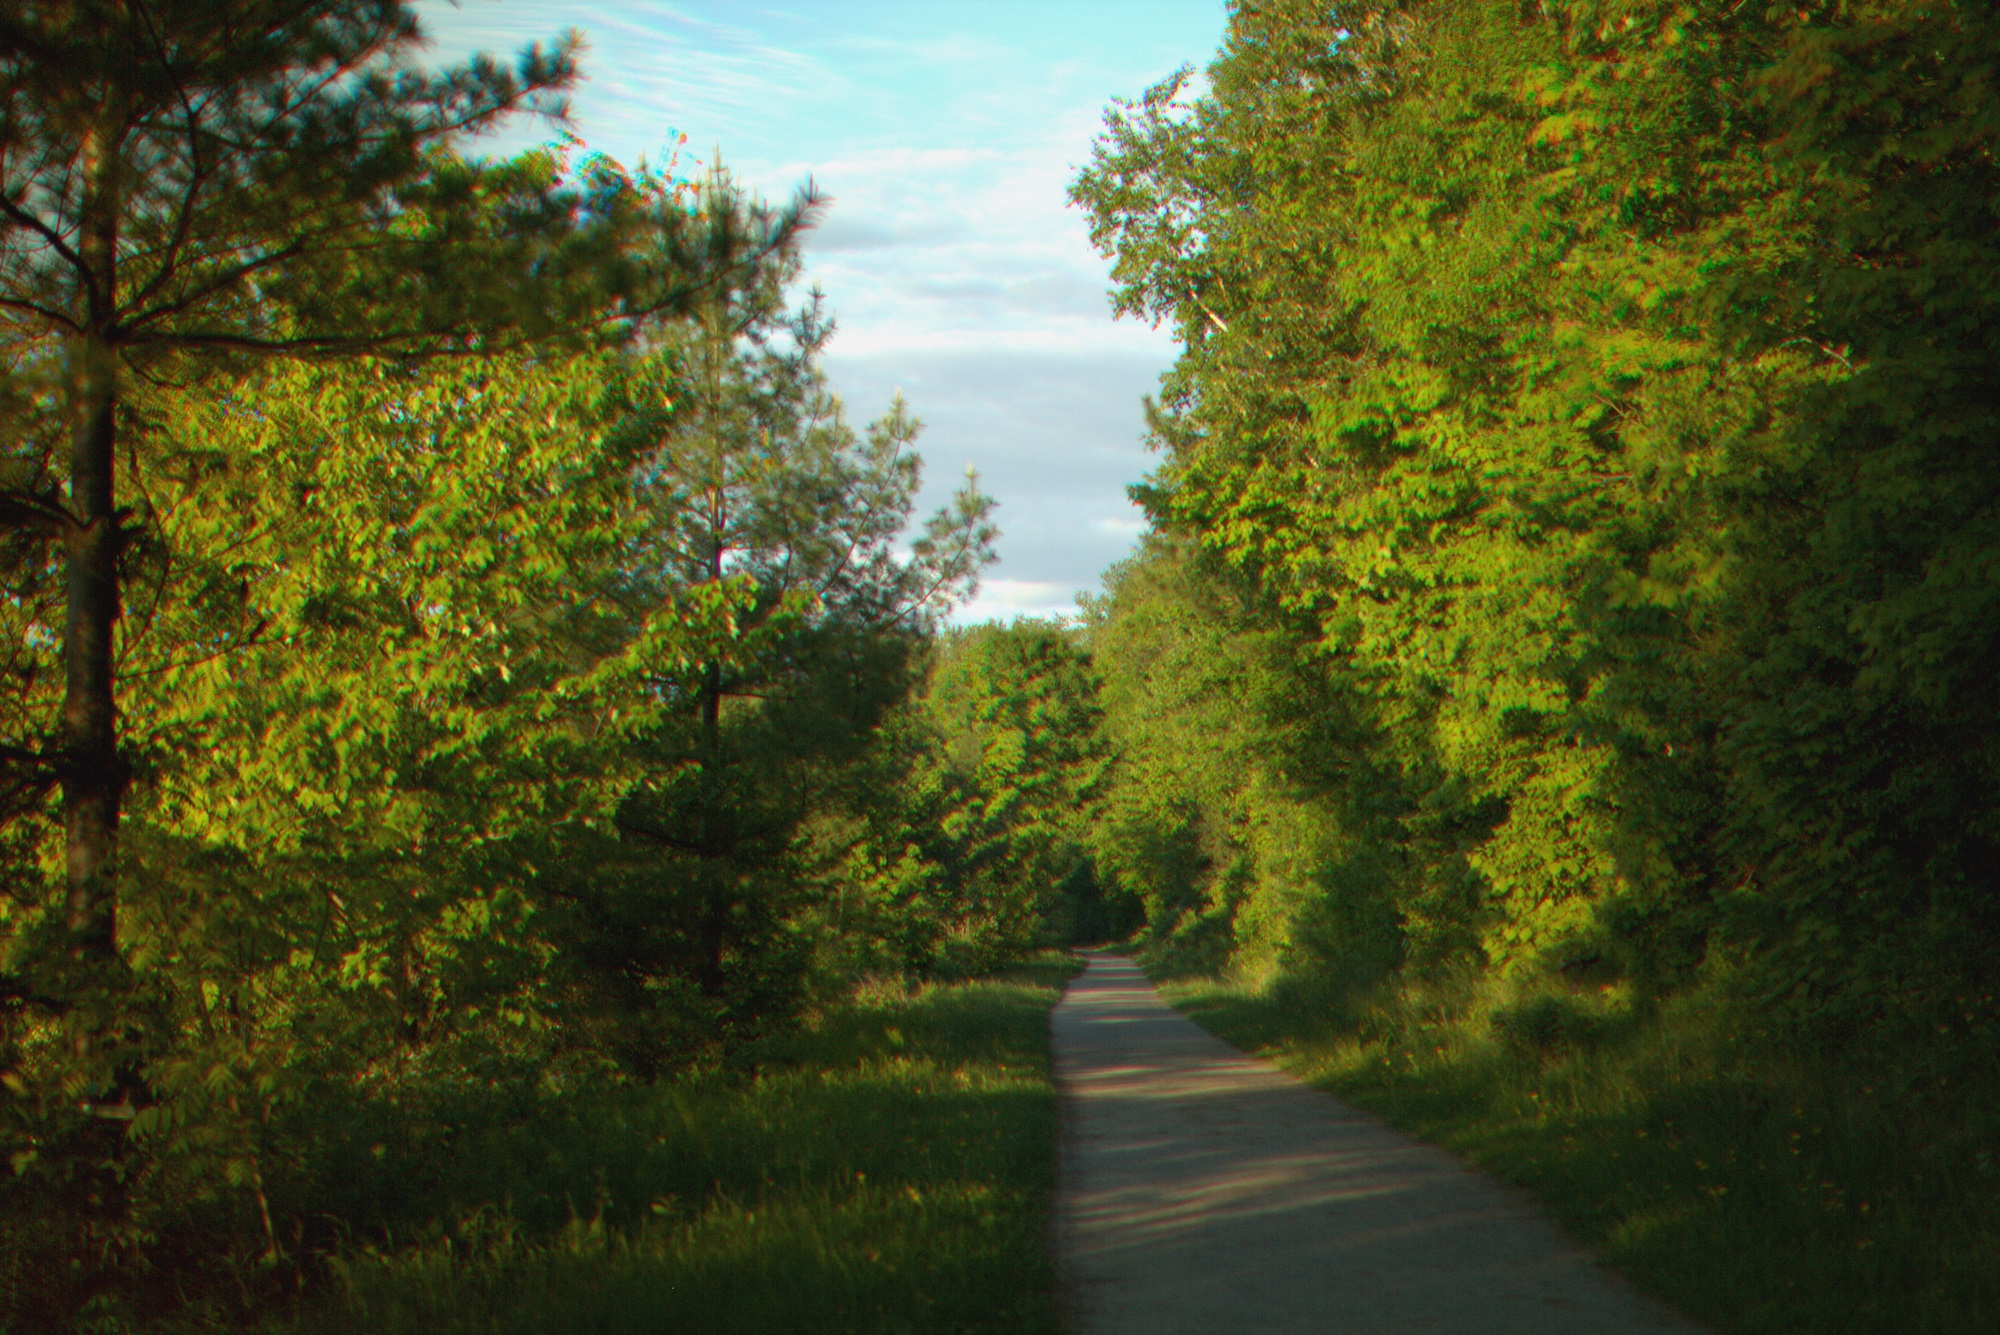
\includegraphics[width=0.30\linewidth]{vermont_path.jpg}
%  \caption{Reconstructed image of Vermont landscape at sunset; f/2.8, ISO 200, 1/200 sec.}
%%  \label{path_mesh}
%  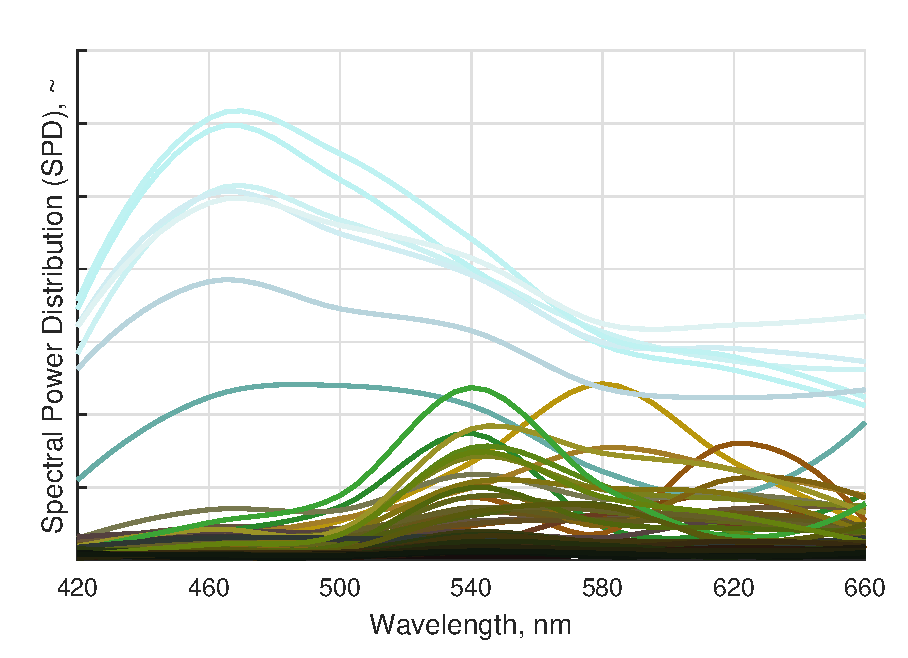
\includegraphics[width=0.30\linewidth]{vermont_path.eps}
%  \caption{SPDs and reconstructed colors sampled at a 70-node square mesh for the scene in Figure \ref{path_mesh}.}
%  \label{path_SPDs}
%  \end{centering}
%\end{figure}

%%%%%%%%%%%%%%%%%%%%%%%%%%%%

\clearpage
\twocolumn

\section{Discussion}

This paper demonstrates a method for high-resolution visible light spectral imaging at less than 10\% the cost of a commercial hyperspectral camera, using only commercially-available hardware. Results are validated quantitatively and qualitatively against ground truth. Key aspects of novelty include characterization of SPD dimensionality, curve reconstruction from sparse samples, and fusion of trichromate measurements. This method significantly improves access to the field of spectral imaging, and enables further research into the field of spectral image processing.

%\id Observer functions $[ \bar{x}, \bar{y}, \bar{z} ]$ have inherent limitations as the sole basis for generating RGB images from HSDCs. They model independent single-color perception only, and do not account for the the mutual influence of simultaneously-perceived colors. This deficiency is apparent in complex scenes where SPDs span several orders of magnitude, or the illuminant is significantly non-spectrally uniform, i.e.\ colored.

%\id Future work may include:
%
%\begin{enumerate}
%\item Quantifying the mutual perceptual influence of colors
%\item Reducing the diameter of the lens objective and filters 
%\item Improving and/or automating the filter cycling
%\item Quantifying absolute sensor response to dimensionalize SPDs
%\end{enumerate}

\section{Acknowledgements}

The author gratefully recognizes his friends, family, and colleagues for their generous and thoughtful support in shaping this work --- in particular: Eric Kirchner, Trey Henderson, Bronek Dichter, Michał Dichter, and Evan Molinari.

%%%%%%%%%%%%%%%%%%%%%%%%%%%%%%%%%%%%%%%%%%%%%%%%%%%%%%%%%%%%

 \begin{thebibliography}{12}

\bibitem{BabelColor}
{BabelColor. \emph{The ColorChecker Pages}. Accessed 2021-08-01. https://www.babelcolor.com}

\bibitem{Baek}
{Baek, S.-H., Kim, I., Gutierrez, D., \& Kim, M. H. (2017). \emph{Compact Single-Shot Hyperspectral Imaging Using a Prism.} ACM Transactions on Graphics, 36(6), 1–12. https://doi.org/10.1145/3130800.3130896}

\bibitem{Berns}
{Berns, R., Taplin, L., Nezamabadi, M., Mohammadi, M., \& Zhao, Y. (2005). \emph{Spectral imaging using a commercial color-filter array digital camera.}}

\bibitem{dcraw}
{Coffin, D. \emph{Decoding raw digital photos in Linux}. (n.d.). https://www.dechifro.org/dcraw/.}

\bibitem{CVRL}
{Colour \& Vision Research Laboratory (n.d.). \emph{CVRL Main.} http://cvrl.ioo.ucl.ac.uk/index.htm.}

\bibitem{Cosentino}
{Cosentino, A. (2015). \emph{Multispectral Imaging System Using 12 Interference Filters for Mapping Pigments.} Conservar Património, 21, 25–38. https://doi.org/10.14568/cp2015005}

\bibitem{Habel}
{Habel, R., Kudenov, M., \& Wimmer, M. (2012). \emph{Practical Spectral Photography.} Computer Graphics Forum, 31(2pt2), 449–458. https://doi.org/10.1111/j.1467-8659.2012.03024.x}

\bibitem{Jiang}
{Jiang, J., Liu, D., Gu, J., \& Susstrunk, S. (2013). \emph{What is the Space of Spectral Sensitivity Functions for Digital Color Cameras?} 2013 IEEE Workshop on Applications of Computer Vision (WACV). https://doi.org/10.1109/wacv.2013.6475015}

\bibitem{Lindbloom}
{Lindbloom, B. J. (n.d.). \emph{Spectral Computation of XYZ.} http://www.brucelindbloom.com.}

\bibitem{Oh}
{Oh, S. W., Brown, M. S., Pollefeys, M., \& Kim, S. J. (2016). \emph{Do It Yourself Hyperspectral Imaging with Everyday Digital Cameras.} 2016 IEEE Conference on Computer Vision and Pattern Recognition (CVPR). https://doi.org/10.1109/cvpr.2016.270}

 \bibitem{Parkkinen} 
 {Parkkinen, J. P. S., Hallikainen, J., \& Jaaskelainen, T. (1989, February 1). \emph{Characteristic Spectra of Munsell Colors}. JOSA A.}

\bibitem{Thorlabs}
{Thorlabs. \emph{UV/VIS Bandpass \& Laser Line Filters: 340 - 694.3 nm Center Wavelength}. Accessed 2020-10-19. https://www.thorlabs.com.}

\bibitem{X-Rite}
{X-Rite. \emph{Colorimetric values for ColorChecker family of targets}. 2019-04-11. https://xritephoto.com.}

\end{thebibliography}
 
%\begin{table}[t]
%\begin{center}
%\begin{tabular}{l l r}
%\textbf{Item} & \textbf{Vendor} & \textbf{Cost, \$} \\
%\hline
%Spectro 1 spectrophotometer       & Variable, Inc. &   325 \\
%Canon 650D camera                 & eBay &             300 \\
%Canon EF 40 mm prime lens         & Canon &            150 \\
%Thorlabs FB420-10 1''      & Thorlabs &         108 \\
%Thorlabs FB460-10 1''      & Thorlabs &         102 \\
%Thorlabs FB500-10 1''      & Thorlabs &         100 \\
%Thorlabs FB540-10 1''      & Thorlabs &         94  \\
%Thorlabs FB580-10 1''      & Thorlabs &         94  \\
%Thorlabs FB620-10 1''      & Thorlabs &         94  \\
%Thorlabs FB660-10 1''      & Thorlabs &         94  \\
%Thorlabs BX0110 case  & Thorlabs &         29  \\
%X-Rite ColorChecker Classic         & B\&H Photo Video & 80  \\
%Velbon VideoMate II tripod        & eBay &             33  \\
%Velbon QB-5RL mount & Amazon &           17  \\
%Neewer remote shutter             & Amazon &           23  \\
%\hline
%\textbf{Total, all items} & & 1,643 \\
%\textbf{Total, filters only} & & 715 \\
%\end{tabular}
%\caption{Bill of materials.}
%\label{materials}
%\end{center}
%\end{table}
 
 %%%%%%%%%%%%%%%%%%%%%%%%%%%%%%%%%%%%%%%%%%%%%%%%%

%\clearpage 
%\onecolumn
%\section{Appendices}

%\begin{figure}[H]
%\begin{centering}
%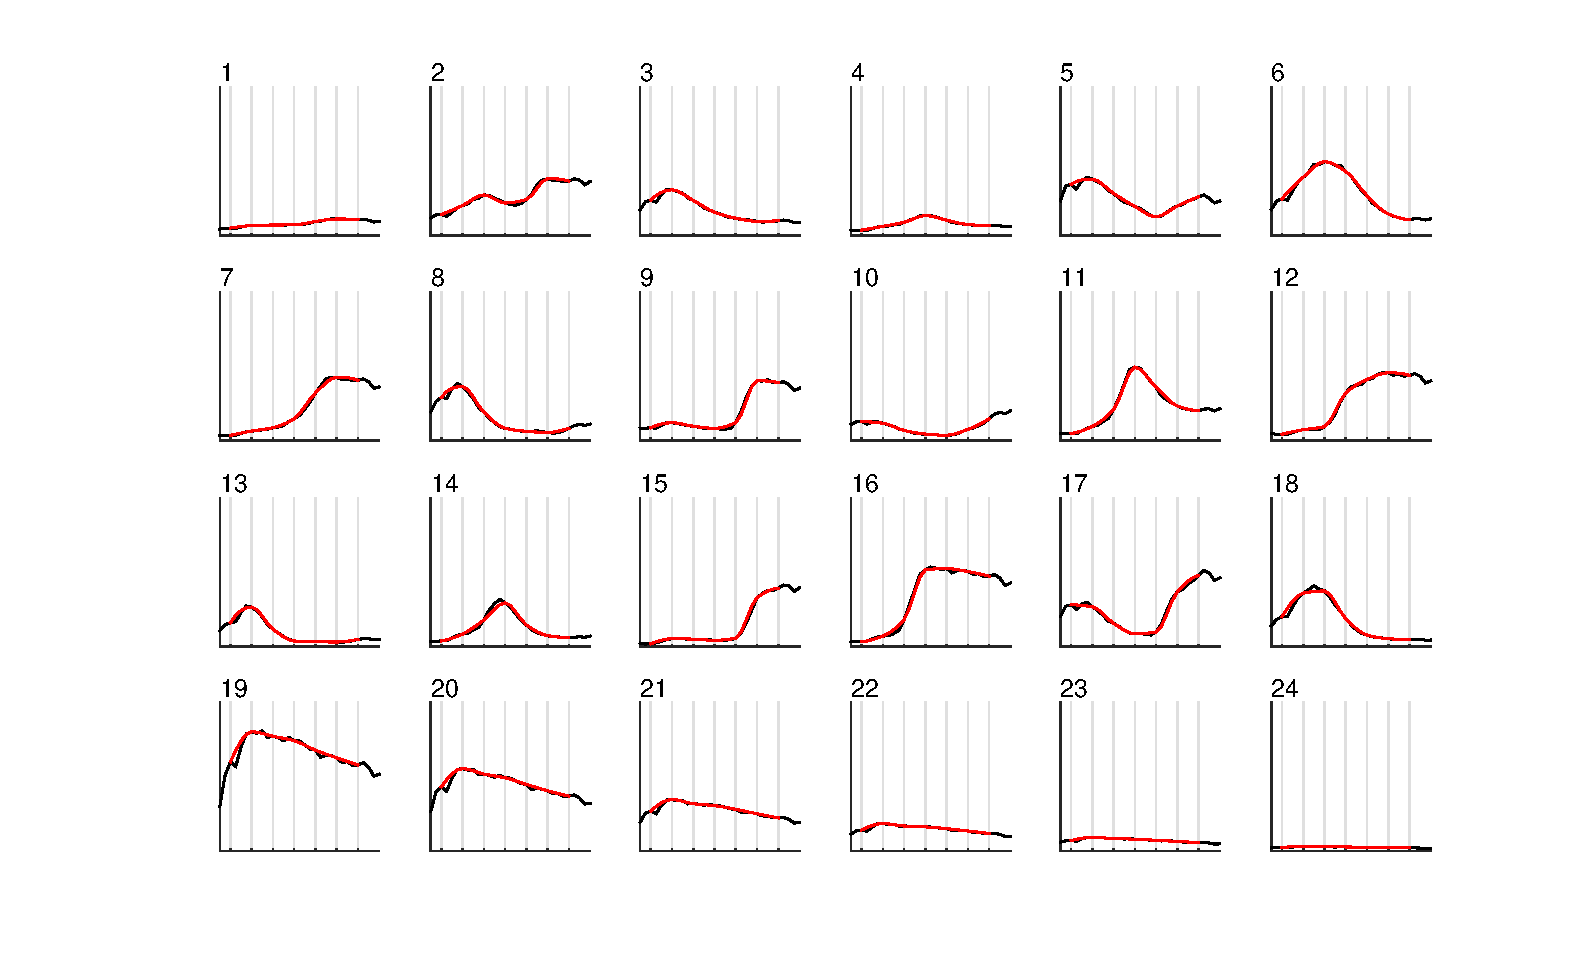
\includegraphics[width=0.90\textwidth]{colorchecker_reconstruction.eps}
%\caption{Curve reconstruction of simulated non-dimensional ColorChecker SPDs, modeled as measured reflectance spectra under D65 illuminant, with cubic interpolation, seven samples, 40 nm resolution, over 420 to 660 nm.}
%\label{colorchecker_reconstruction}
%\end{centering}
%\end{figure}

%\begin{figure}[H]
%\centering
%  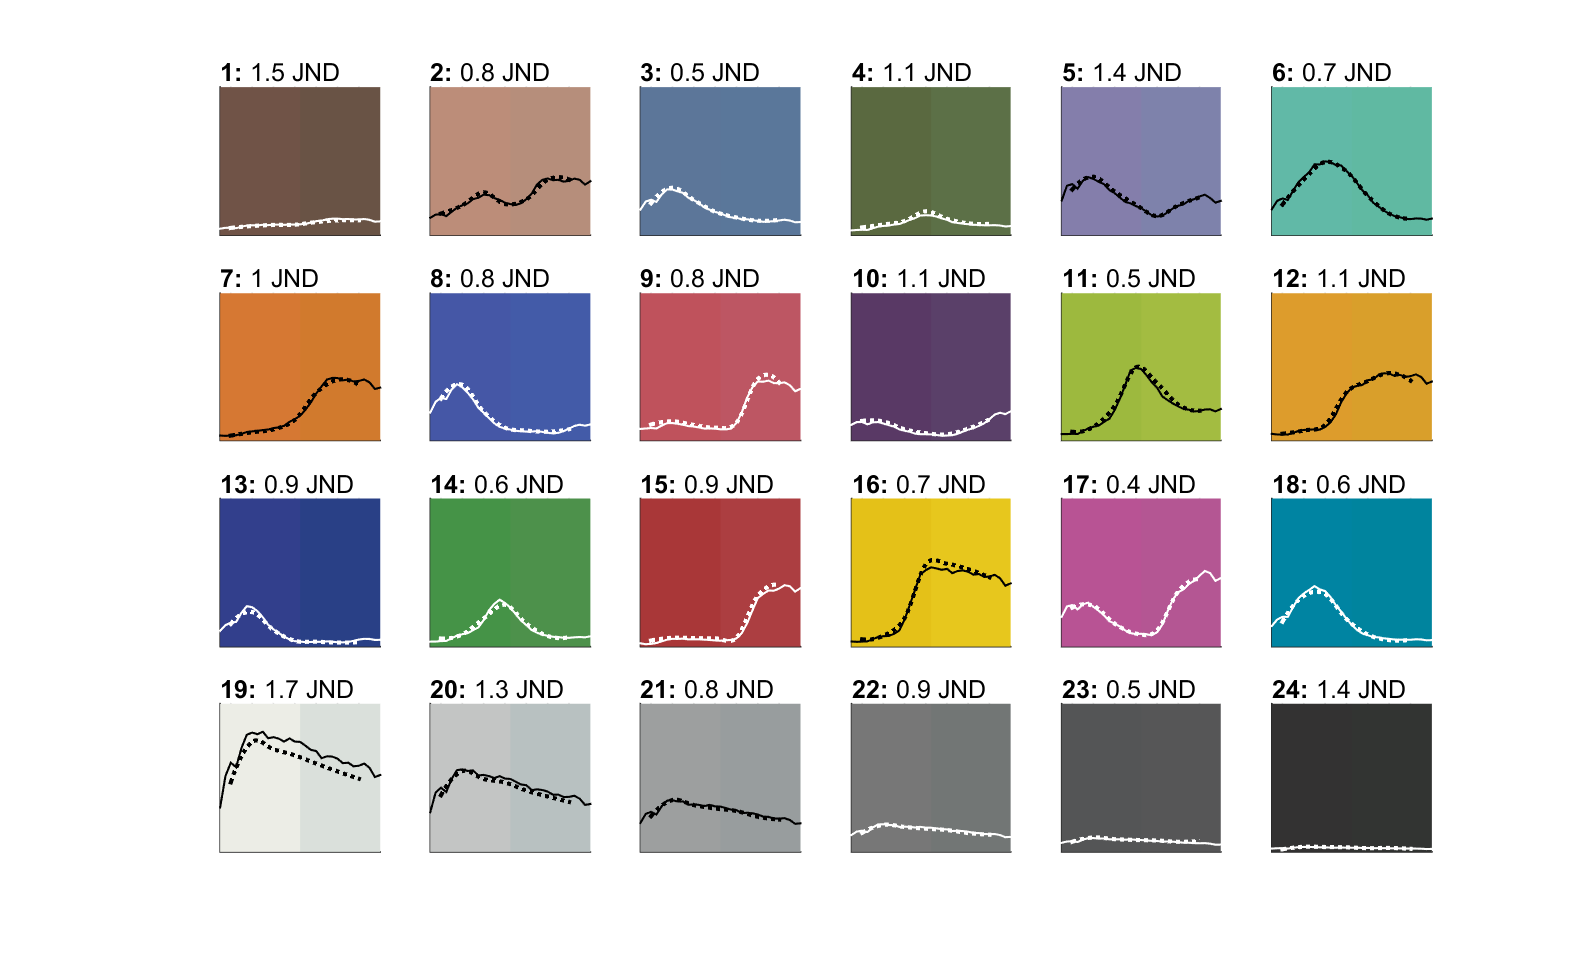
\includegraphics[width=0.90\linewidth]{SPD_validation.eps}
%  \caption{Comparison of SPDs and colors as measured by spectrophotometer (solid, left) and camera (dashed, right). A single scalar gain is applied to align the magnitudes of the two sets of curves. Color error in CIEDE2000 is reported for each swatch. Plots are scaled 400 to 700 nm along x, and non-dimensional along y.}
%  \label{SPD_validation}
%\end{figure}

\end{document}


